%%%%%%%%%%%%%%%%%%%%%%%%%%%%%%%%%%%%%%%%%%%%%%%%%%%%%%%%%%%%%%%%%%%%%
%% This is a (brief) model paper using the achemso class
%% The document class accepts keyval options, which should include
%% the target journal and optionally the manuscript type. 
%%%%%%%%%%%%%%%%%%%%%%%%%%%%%%%%%%%%%%%%%%%%%%%%%%%%%%%%%%%%%%%%%%%%%
\documentclass[journal=aesccq,manuscript=draft]{achemso}
\usepackage{amsmath}
\usepackage{placeins}
\usepackage{comment}
\usepackage{amssymb}

\usepackage{ulem}


%%%%%%%%%%%%%%%%%%%%%%%%%%%%%%%%%%%%%%%%%%%%%%%%%%%%%%%%%%%%%%%%%%%%%
%% Place any additional packages needed here.  Only include packages
%% which are essential, to avoid problems later. Do NOT use any
%% packages which require e-TeX (for example etoolbox): the e-TeX
%% extensions are not currently available on the ACS conversion
%% servers.
%%%%%%%%%%%%%%%%%%%%%%%%%%%%%%%%%%%%%%%%%%%%%%%%%%%%%%%%%%%%%%%%%%%%%
\usepackage[version=3]{mhchem} % Formula subscripts using \ce{}
\usepackage{tikz} % For legend line drawings


%%%%%%%%%%
% Line stlye defs for Reaction Contribution Plots legend
%%%%%%%%%%

%\newcommand{\tikzSolidLine}[]{\tikz[baseline=-.7ex]{\draw[thick, solid](0,0)--(1,0);}}

\newcommand{\tikzSolidLine}{
    \begin{tikzpicture}[baseline={([yshift=-.6ex]current bounding box.center)}]    
      \draw[thick, solid] (0,0) -- (1,0);
    \end{tikzpicture}{}
}

\newcommand{\tikzDottedLine}{
    \begin{tikzpicture}[baseline={([yshift=-.6ex]current bounding box.center)}]        
      \draw[thick, dotted] (0,0) -- (1,0);
    \end{tikzpicture}{}
}

\newcommand{\tikzDashedLine}{
    \begin{tikzpicture}[baseline={([yshift=-.6ex]current bounding box.center)}]       
      \draw[thick, dashed] (0,0) -- (1,0);
    \end{tikzpicture}{}
}

\newcommand{\tikzDashDottedLine}{
    \begin{tikzpicture}[baseline={([yshift=-.6ex]current bounding box.center)}]       
      \draw[thick, dashdotted] (0,0) -- (1,0);
    \end{tikzpicture}{}
}

\newcommand{\tikzDashThreeDottedLine}{
    \begin{tikzpicture}[dash pattern=on 3pt off 2pt on 1pt off 2pt on 1pt off 2pt on 1pt off 2pt,baseline={([yshift=-.6ex]current bounding box.center)}]      
      \draw[thick] (0,0) -- (1,0);
    \end{tikzpicture}{}
}

\setcounter{secnumdepth}{4} % For /paragraph{} numbering 

\usepackage{caption}    % For subfigures
\usepackage{subcaption} % For subfigures


%%%%%%%%%%%%%%%%%%%%%%%%%%%%%%%%%%%%%%%%%%%%%%%%%%%%%%%%%%%%%%%%%%%%%
%% If issues arise when submitting your manuscript, you may want to
%% un-comment the next line.  This provides information on the
%% version of every file you have used.
%%%%%%%%%%%%%%%%%%%%%%%%%%%%%%%%%%%%%%%%%%%%%%%%%%%%%%%%%%%%%%%%%%%%%
%%\listfiles

%%%%%%%%%%%%%%%%%%%%%%%%%%%%%%%%%%%%%%%%%%%%%%%%%%%%%%%%%%%%%%%%%%%%%
%% Place any additional macros here.  Please use \newcommand* where
%% possible, and avoid layout-changing macros (which are not used
%% when typesetting).
%%%%%%%%%%%%%%%%%%%%%%%%%%%%%%%%%%%%%%%%%%%%%%%%%%%%%%%%%%%%%%%%%%%%%
\newcommand*\mycommand[1]{\texttt{\emph{#1}}}

%Reaction counter for photoprocesses
\newcounter{pcounter}
\newcommand{\pcount}[1]{\refstepcounter{pcounter}\label{#1}\ref{#1}}
\renewcommand\thepcounter{P\arabic{pcounter}}

%Reaction counter for reactions
\newcounter{ncounter}
\newcommand{\ncount}[1]{\refstepcounter{ncounter}\label{#1}\ref{#1}}
\renewcommand\thencounter{N\arabic{ncounter}}


%%%%%%%%%%%%%%%%%%%%%%%%%%%%%%%%%%%%%%%%%%%%%%%%%%%%%%%%%%%%%%%%%%%%%
%% Meta-data block
%% ---------------
%% Each author should be given as a separate \author command.
%%
%% Corresponding authors should have an e-mail given after the author
%% name as an \email command. Phone and fax numbers can be given
%% using \phone and \fax, respectively; this information is optional.
%%
%% The affiliation of authors is given after the authors; each
%% \affiliation command applies to all preceding authors not already
%% assigned an affiliation.
%%
%% The affiliation takes an option argument for the short name.  This
%% will typically be something like "University of Somewhere".
%%
%% The \altaffiliation macro should be used for new address, etc.
%% On the other hand, \alsoaffiliation is used on a per author basis
%% when authors are associated with multiple institutions.
%%%%%%%%%%%%%%%%%%%%%%%%%%%%%%%%%%%%%%%%%%%%%%%%%%%%%%%%%%%%%%%%%%%%%
\author{Kristen Darnell}
\affiliation[San Jose State University]{Department of Astronomy, San Jose State University, San Jose, California, USA}
\author{Daniel Lopez-Sanders}
\affiliation[Benedictine College]{Department of Physics and Astronomy, Benedictine College, Atchison, KS, USA}

\author{Others}

\author{Christopher N. Shingledecker}
\affiliation[VMI]{Department of Chemistry, Virginia Military Institute, Lexington, VA 24450 USA}
\email{shingledeckercn@vmi.edu}
\phone{+1 (540) 464-7422}


%%%%%%%%%%%%%%%%%%%%%%%%%%%%%%%%%%%%%%%%%%%%%%%%%%%%%%%%%%%%%%%%%%%%%
%% The document title should be given as usual. Some journals require
%% a running title from the author: this should be supplied as an
%% optional argument to \title.
%%%%%%%%%%%%%%%%%%%%%%%%%%%%%%%%%%%%%%%%%%%%%%%%%%%%%%%%%%%%%%%%%%%%%
\title[Ion-Ice Reactions in Astrochemistry]
  {Ion-Ice Reactions in Astrochemical Models}

%%%%%%%%%%%%%%%%%%%%%%%%%%%%%%%%%%%%%%%%%%%%%%%%%%%%%%%%%%%%%%%%%%%%%
%% Some journals require a list of abbreviations or keywords to be
%% supplied. These should be set up here, and will be printed after
%% the title and author information, if needed.
%%%%%%%%%%%%%%%%%%%%%%%%%%%%%%%%%%%%%%%%%%%%%%%%%%%%%%%%%%%%%%%%%%%%%
\abbreviations{}
\keywords{Astrochemistry, Ion-neutral reactions}

%%%%%%%%%%%%%%%%%%%%%%%%%%%%%%%%%%%%%%%%%%%%%%%%%%%%%%%%%%%%%%%%%%%%%
%% The manuscript does not need to include \maketitle, which is
%% executed automatically.
%%%%%%%%%%%%%%%%%%%%%%%%%%%%%%%%%%%%%%%%%%%%%%%%%%%%%%%%%%%%%%%%%%%%%
\begin{document}

%%%%%%%%%%%%%%%%%%%%%%%%%%%%%%%%%%%%%%%%%%%%%%%%%%%%%%%%%%%%%%%%%%%%%
%% The "tocentry" environment can be used to create an entry for the
%% graphical table of contents. It is given here as some journals
%% require that it is printed as part of the abstract page. It will
%% be automatically moved as appropriate.
%%%%%%%%%%%%%%%%%%%%%%%%%%%%%%%%%%%%%%%%%%%%%%%%%%%%%%%%%%%%%%%%%%%%%
\begin{tocentry}

Some journals require a graphical entry for the Table of Contents.
This should be laid out ``print ready'' so that the sizing of the
text is correct.

Inside the \texttt{tocentry} environment, the font used is Helvetica
8\,pt, as required by \emph{Journal of the American Chemical
Society}.

The surrounding frame is 9\,cm by 3.5\,cm, which is the maximum
permitted for  \emph{Journal of the American Chemical Society}
graphical table of content entries. The box will not resize if the
content is too big: instead it will overflow the edge of the box.

This box and the associated title will always be printed on a
separate page at the end of the document.

\end{tocentry}

%%%%%%%%%%%%%%%%%%%%%%%%%%%%%%%%%%%%%%%%%%%%%%%%%%%%%%%%%%%%%%%%%%%%%
%% The abstract environment will automatically gobble the contents
%% if an abstract is not used by the target journal.
%%%%%%%%%%%%%%%%%%%%%%%%%%%%%%%%%%%%%%%%%%%%%%%%%%%%%%%%%%%%%%%%%%%%%
\begin{abstract}
    In astrochemistry, gas-phase ion-neutral reactions have been known to be of 
    central importance for the formation of polyatomic molecules since the first 
    pioneering models of the chemical evolution of interstellar environments. Later,
    it was similarly realized that the ice mantles of interstellar dust grains are
    also critical for understanding chemical complexity in space. Nevertheless, there 
    are as yet no models which seek to elucidate what, if any, role ion-neutral reactions 
    play in these dust-grain ice mantles, so-called ``ion-ice'' chemistry. In this work, we present results of our study to investigate this topic. Rather than beginning with the simulation of
    an interstellar source, we model the chemical evolution of a dust-grain ice analogue of
    pure oxygen, and compare the results of our calculation with previous experimental
    data. The results of these preliminary studies suggest that, as in the gas-phase, 
    ion-ice chemistry may be similarly important for understanding the chemical composition
    of molecules on grains, including potentially species implicated in the origin of life. 
\end{abstract}

%%%%%%%%%%%%%%%%%%%%%%%%%%%%%%%%%%%%%%%%%%%%%%%%%%%%%%%%%%%%%%%%%%%%%
%% Start the main part of the manuscript here.
%%%%%%%%%%%%%%%%%%%%%%%%%%%%%%%%%%%%%%%%%%%%%%%%%%%%%%%%%%%%%%%%%%%%%
\section{Introduction}

The year 2023 marked the 50$^{th}$ anniversary of the field of astrochemical modeling, which began with the pioneering work of \citet{herbst_formation_1973}. A number of key  predictions from that work have since been verified in the intervening years. Among these was the claim that ion-neutral reactions - beginning with those involving \ce{H3+} - were essential to the  formation of polyatomic molecules in interstellar environments, given the fact that they are very often barrierless and exothermic, which allows them to proceed efficiently even at the low temperatures of cold molecular clouds, which are often around 10 K (See the recent review by \citet{ceccarelli_organic_2022} and references therein for more details). In addition, especially for cases the neutral species is polar, the long-range forces involved mean that such reactions can actually have a negative temperature  dependence \citep{woon_quantum_2009}, and can have rate coefficients significantly larger than that predicted by collision theory of $\sim10^{-10}$ cm$^3$ s$^{-1}$ \citep{hammes_principles_1978}. 

A far later development has been the ongoing realization of the importance of dust-grain ice mantles in explaining the observed chemical complexity of interstellar environments, particularly in the case of Terrestrial-like saturated or semi-saturated organic species, including ``prebiotic'' molecules which may be implicated in the origins of life on Earth and possibly elsewhere \citep{ceccarelli_organic_2022}. Nevertheless, the addition of surface and bulk ice-mantle grain chemistry - though doubtless a more accurate representation of chemistry in the real interstellar medium - poses a number of distinct challenges for astrochemical models.

The rather unfortunate combination of the importance of grain-related processes in the ISM, combined with a comparative lack of knowledge and data regarding relevant processes, led one astrochemical modeler to make the now well-known jest that interstellar grain chemistry represents the ``last refuge of the scoundrel\citep{charnley_molecular_1992}.'' Here, we will highlight just a few of the current areas of uncertainty that pose challenges for modeling. First, there exits substantial uncertainties regarding the physisorption binding energies of most of the hundreds of species usually included in grain-chemical networks \citep{cuppen_modelling_2011,lamberts_influence_2017,wakelam_binding_2017}, and these binding energies, which in fact have a range of values depending on, e.g., the local surface morphology, are typically approximated with a single value except in some very recent studies \citep{grassi_novel_2020}. Moreover, though it is now well established both via experiments and theory that grain and ice-mantle surface chemistry is dominated by diffusive Langmuir-Hinshelwood type reactions \citep{qasim_experimental_2020,ioppolo_non-energetic_2020,cuppen_grain_2017,watanabe_efficient_2002}, how - or indeed whether - chemistry within the ice mantle occurs at low temperatures has been the subject of considerable recent work, though there is a growing consensus that non-diffusive processes almost certainly play a key role \citep{theule_thermal_2013,ghesquiere_diffusion_2015,shingledecker_simulating_2019}. Finally, and most germane for this work, the chemical networks used for simulating interstellar grain chemistry invariably include only neutral species.

That ion-ice processes can occur efficiently under interstellar conditions was suggested in the pioneering theoretical study of \citet{woon_ion-ice_2011}, who found that, e.g., cations such as \ce{HCO+} and \ce{CH3+} were able to react barrierlessly with water molecules in an ice via pathways that could lead to formic acid and methanol, two astrochemically-relevant species. The reaction between low-energy \ce{CH3+} cations and water ice was elegantly investigated in detail by \citet{nakai_methanol_2023}, who confirmed experimentally that the reaction suggested by \citet{woon_ion-ice_2011} does indeed occur under interstellar conditions. In that work, astrochemical models using the code of \citet{furuya_water_2015} found that the \ce{CH3+}-ice reaction was competitive at the edges of the simulated molecular cloud, where the model predicted enhanced abundances of gas-phase \ce{CH3+}. 

The adsorption of gas-phase cations undoubtedly occurs in real interstellar environments; however, there exist other mechanisms for driving ion-ice chemistry. Though externally produced energetic photons are quickly extinquished in molecular clouds, galactic cosmic rays can penetrate essentially the entirety of such regions, and are an important source of continuous ice processing in the ISM \citep{strazzulla_ion_2009,dartois_cosmic_2018}. The essential role of comsic rays to astrochemistry was recognized even in the first model of \citet{herbst_formation_1973}, who noted that it drives the formation of \ce{H3+}. Cosmic ray collisions with \ce{H2} can also produce an internal flux of UV photons, which can further ionize species in the cloud \citep{prasad_uv_1983,padovani_ultraviolet_2024}. Cosmic ray collisions with dust grains and their ice mantles similarly result in the formation of charged species within a roughly cylindrical region known as the ``track'' \citep{shingledecker_cosmic-ray_2020}. Bombardment by UV photons represents another means of forming internal ions \citep{mullikin_new_2021}, albeit with a lower efficiency than with cosmic rays \citep{wu_role_2024}. Some fraction of the charged species produced within ices undergo rapid neutralization by recombination \citep{shingledecker_general_2018,woon_formation_2024}; however, the remainder may participate in an internal ion-ice chemistry whose importance may be comparable to that known to occur in the gas-phase. 

In this work, we present the first computational study of ion-ice chemistry driven by the bombardment of a cosmic ice analogue by UV photons. Our paper is laid out as follows: in \S\ref{sec:theory} we describe our theoretical and computational approach, in \S\ref{sec:results} we present the results of our models and describe their astrochemical significance, and finally, \S\ref{sec:conclusions} summarizes our findings. 

\section{Theory} \label{sec:theory}

\subsection{Formation of Ions Within Cosmic Ice}\label{sec:ionformation}

In this work, we are focused on the chemical contribution of ions produced within cosmic ice. In dense molecular clouds, there exist two main mechanisms which could drive the ionization of dust-grain ice mantle species; namely, galactic cosmic rays\citep{silsbee_magnetic_2018,ivlev_penetration_2018} and the UV photons they generate through the excitation of \ce{H2}\citep{prasad_uv_1983}. The basis of the theoretical approach used in our models is that of \citet{shingledecker_general_2018}, which begins with the assumption of a set of four possible outcomes when some ice constituent, \ce{A}, encounters some particle of ionizing radiation:

\begin{equation}
aA \leadsto{} aA^+ + e^-
\tag{R1}
\label{r1}
\end{equation}

\begin{equation}
aA \leadsto{} aA^+ + e^- \rightarrow{} aA^* \rightarrow{} bB^* + cC^*
\tag{R2}
\label{r2}
\end{equation}

\begin{equation}
aA \leadsto{} aA^* \rightarrow{} bB + cC
\tag{R3}
\label{r3}
\end{equation}

\begin{equation}
aA \leadsto{} aA^*
\tag{R4}
\label{r4}
\end{equation}

\noindent
where the lower case letters represent the relevant stoichiometric coefficients. Processes \eqref{r1} and \eqref{r2} correspond to the ionization of \ce{A}, while \eqref{r3} and \eqref{r4} represent the effects of excitation to a higher vibrational or electronic state. \citet{shingledecker_general_2018} furthermore derive expressions for the rate coefficients \eqref{r1} - \eqref{r4}, albeit for cases where the \ce{A} encounters a particle such as an energetic proton. This formalism was later expanded by \citet{mullikin_new_2021}, where the corresponding photo ionization or excitation rate coefficients were derived for \eqref{r1} - \eqref{r4}, which is what is used here. 

In large part because grain-chemical networks have only included neutral species, previous modeling works using one of the above approaches have made the assumption that in every case, the ionization of \ce{A} proceeds via \eqref{r2} rather than \eqref{r1}, i.e., that ionization is followed by rapid charge recombination to yield some excited suprathermal products. Conversely, in this work, we assume for the first time that \eqref{r1} and \eqref{r2} occur with equal probability, thereby allowing for the explicit formation of ions within the ice.

Briefly, to obtain rate coefficients for \eqref{r1} - \eqref{r4}, we begin with the standard formula for photo-processes:

\begin{equation}
    k_\mathrm{photo} = \int \sigma(\lambda)I(\lambda) d\lambda
    \label{eq:kphotostandard}
\end{equation}

\noindent  
where the resulting value is a function of the wavelength-dependent absorption cross-sections, $\sigma(\lambda)$ and intensities, $I(\lambda)$, integrated over all wavelengths \citep{van_dishoeck_photodissociation_1988}. To obtain the ultimately-utilized expression for the rate coefficients, we express Eq. \eqref{eq:kphotostandard} as

\begin{equation}
    k_\mathrm{photo} = \frac{\int \sigma(\lambda)I(\lambda)d\lambda}{\int I(\lambda)d\lambda} \int I(\lambda)d\lambda = \Bar{\sigma}\Phi
    \label{eq:kmullikin}
\end{equation}

\noindent
such that, as shown in Eq. \eqref{eq:kmullikin}, the rate coefficient can be written as the product of an average cross section for a given species and the photon flux. 

As given in \citet{mullikin_new_2021}, the individual $k_\mathrm{photo}$ values for \eqref{r1} - \eqref{r4} are then multiplied by some branching fractions, $f_\mathrm{br}$, which as in that work, we take to be equal. In addition, that work further adds an additional factor, $\delta$, which accounts for any discrepancy between, e.g., the actual solid phase cross-sections compared with the gas-phase values used here. Thus, the rate coefficients for photo-driven processes in our model is,

\begin{equation}
    k_\mathrm{photo} = f_\mathrm{br}\Bar{\sigma}\Phi\delta.
\end{equation}

\noindent
Shown in Table \ref{tbl:network_photo} are the cross sections and associated $\delta$-values for the various processes used here, taken from \citet{mullikin_new_2021}.

\begin{comment}
\begin{table}
  \caption{Cross-sections and $\delta$-values used in this work for pure O2 ice irradiated by UV photons. Data taken from \citet{mullikin_new_2021}. NOTE: THIS TABLE NEEDS TO BE UPDATED TO INCLUDE IONIC PRODUCTS OF PHOTODISSOCIATION}
  \label{tbl:mullikindata}
  \begin{tabular}{llll}
    \hline
    Process & $\sigma$ (cm$^{-2}$) & $\delta$ \\
    \hline
$\ce{O} + h\nu \rightarrow{} \ce{O}^*$ & 0  & 1.0  \\
$\ce{O} + h\nu \rightarrow{} \ce{O}^*$ & 0  & 1.0 \\
$\ce{O2} + h\nu \rightarrow{} \ce{O^{*}} + \ce{O^{*}}$  & $3.86\times10^{-20}$ & 1.0  \\
$\ce{O2} + h\nu \rightarrow{} \ce{O} + \ce{O}$  & $2.13\times10^{-18}$ & 2.3  \\
$\ce{O2} + h\nu \rightarrow{} \ce{O2^{*}}$  & $2.13\times10^{-18}$ & 1.0  \\
$\ce{O3} + h\nu \rightarrow{} \ce{O2^{*}} + \ce{O^{*}}$  & 0  & 1.0  \\
$\ce{O3} + h\nu \rightarrow{} \ce{O2} + \ce{O}$  & $5.60\times10^{-18}$ & 1.0  \\
$\ce{O3} + h\nu \rightarrow{} \ce{O3^{*}}$  & $5.60\times10^{-18}$ & 1.0 \\
    \hline
  \end{tabular}
\end{table}
\end{comment}

\begin{table}
  \caption{Photoprocesses}
  \label{tbl:network_photo}
 \begin{tabular}{l c c l  c  c  c }
 \hline
 && Reaction &  & Branching Fraction & Cross Section & $\delta$ \\ 
 \hline
 % 8287 & 
 \pcount{plabel1} & \ce{O} & $\leadsto$ & \ce{O^*} &
 1.00E+00 & 0.00E+00 & 1.00E+00 \\
 %%%
 % 8289 &
 \pcount{plabel2} & \ce{O}  & $\leadsto$ & \ce{O+} + \ce{e-} &
 1.00E+00 & 0.00E+00 & 1.00E+00 \\
 %%%
 % 8297 &
 \pcount{plabel3} & \ce{O2} & $\leadsto$ & \ce{O} + \ce{O} &
 3.33E-01 & 2.13E-18 & 1.00E+01\\
 %%%
 % 8299 &
 \pcount{plabel4} & \ce{O2} & $\leadsto$ & \ce{O+} + \ce{O-} &
 3.33E-01 & 2.13E-18 & 1.00E+01 \\
 %%%
 % 8301 & 
 \pcount{plabel5} & \ce{O2} & $\leadsto$ & \ce{O2^*} &
 3.33E-01 & 2.13E-18 & 1.00E+01 \\
 %%%
 % 8303 &
 \pcount{plabel6} & \ce{O2} & $\leadsto$ & \ce{O^*} + \ce{O^*} & 
 5.00E-01 & 3.86E-20 & 1.00E+01 \\
 %%%
 % 8307 &
 \pcount{plabel7} & \ce{O2} & $\leadsto$ & \ce{O2+} + \ce{e-} &
 5.00E-01 & 3.86E-20 & 1.00E+01\\
 %%%
 % 8323 &
 \pcount{plabel8} & \ce{O3} & $\leadsto$ & \ce{O+} + \ce{O2-} & 
 2.50E-01 & 5.60E-18 & 1.00E+03\\
 %%%
 % 8325 &
 \pcount{plabel9} & \ce{O3} & $\leadsto$ & \ce{O2} + \ce{O} &
 2.50E-01 & 5.60E-18 & 1.00E+03\\
 %%%
 % 8327 &
 \pcount{plabel10} & \ce{O3} & $\leadsto$ & \ce{O2+} + \ce{O-} &
 2.50E-01 & 5.60E-18 & 1.00E+03\\
 %%%
 % 8329 &
 \pcount{plabel11} & \ce{O3} & $\leadsto$ & \ce{O3^*} &
 2.50E-01 & 5.60E-18 & 1.00E+03 \\
 %%%
 % 8333 & 
 \pcount{plabel12} & \ce{O3} & $\leadsto$ & \ce{O2^*} + \ce{O^*} &
 5.00E-01 & 0.00E+00 & 1.00E+00 \\
 %%%
 % 8337 & 
 \pcount{plabel13} & \ce{O3} & $\leadsto$ & \ce{O3+} + \ce{e-} &
 5.00E-01 & 0.00E+00 & 1.00E+00 \\
 \hline
 \end{tabular}
\end{table}


\subsection{The Chemistry of Solid-Phase Ions}

Thus formed within the ice as described in \S\ref{sec:ionformation}, the ions in our simulations are allowed to react chemically. Whether, or by which mechanism, reactions occur in low-temperature cosmic ice is still a matter of ongoing investigation. However, we here assume, as in \citet{shingledecker_simulating_2019}, that rapid reactions can and do occur even at temperatures as low as 5 K, albeit between neighbors, in other words, non-diffusively. This approach was motivated by a now large body of experimental studies showing conclusively that even COMs can be formed via fast solid-phase non-diffusive reactions \citep{abplanalp_study_2016,doddipatla_low-temperature_2021,bergantini_combined_2018,fedoseev_hydrogenation_2022} and, when incorporated into simulations of astrophysical environments, yields predicted abundances of ice-mantle species that have proven to be in general agreement with recent JWST observations \citep{shingledecker_efficient_2020,mcclure_ice_2023,yang_corinos_2022}. 

As described in \citet{shingledecker_simulating_2019}, the fast non-diffusive bulk rate coefficient for some reaction \ce{A + B} is given by

\begin{equation}
    k_\mathrm{fast} = f_\mathrm{br}\left[\frac{\nu_0^\mathrm{A} + \nu_0^\mathrm{B}}{n_\mathrm{bulk}} \right] \mathrm{exp}\left( - \frac{E_\mathrm{act}^{AB}}{T_\mathrm{ice}}\right)
    \label{kfast}
\end{equation}

\noindent
where, where $\nu_\mathrm{A}$ and $\nu_\mathrm{B}$ are the vibrational frequencies of A and B, $n_\mathrm{bulk}$ is the number of species in the ice mantle, exclusive of the surface layers, $E_\mathrm{act}$ is the activation energy, if present, and $T_\mathrm{ice}$ is the ice temperature. Note that here and throughout this work, energies are reported in units of Kelvin (given by the quotient of the energy in, e.g., Joules and the Boltzmann constant). If one of the vibrational frequencies is much larger than the other, for example where $\nu_0^\mathrm{A} \gg \nu_0^\mathrm{B}$, then Eq. \eqref{kfast} can be simplified to

\begin{equation}
    k_\mathrm{fast} \approx f_\mathrm{br}\left[\frac{\nu_\mathrm{n-n}}{n_\mathrm{bulk}} \right] \mathrm{exp}\left( - \frac{E_\mathrm{act}^{AB}}{T_\mathrm{ice}}\right)
    \label{kfast2}
\end{equation}

\noindent
where $\nu_\mathrm{n-n} = \nu_0^\mathrm{A}$. Hereafter, we will refer to $\nu_\mathrm{n-n}$ as the neutral-neutral trial frequency.

As originally described in \citet{shingledecker_simulating_2019}, the species undergoing fast solid-phase reactions were all neutrals. For the purposes of this work, we have modified Eq. \eqref{kfast} slightly to also treat the solid-phase reaction of ions. First, for reactions between ions and neutrals of the form \ce{A+ + B}, we replace $\nu_\mathrm{n-n}$ with another frequency $\nu_\mathrm{i-n}$, the ion-neutral trial frequency. Finally, for reactions between two charged species of the form \ce{A+ + B-}, we invoke a third frequency, $\nu_\mathrm{i-i}$, the ion-ion trial frequency. The use here of these three frequencies in Eq. \eqref{kfast2} comes from the different long-range forces that would be experienced between the reactants which, at least in the case of reactions between a cation and an anion, could increase the overall reaction rate relative over one involving two neutral species, even in an environment where diffusion is severly inhibited. As we describe in \S\ref{sec:results}, these three frquencies were varied in our models to ascertain their influence on the resulting predicted abundances.

\subsection{Model and Chemical Network}

\subsubsection{Reaction Network}

The reaction network, shown in Table \ref{tbl:network_rxn}, in this work was limited to species relevant for a pure \ce{O2} ice. Our starting point was the network in \citet{mullikin_new_2021}, which in turn was based on previous work by \citet{shingledecker_simulating_2019} and \citet{shingledecker_new_2017}. Our base network, which included only reactions between neutral species, was expanded to include ion-neutral reactions of the form

\begin{equation}
    \ce{A+ + B -> C+ + D}
\end{equation}

\noindent
using the reaction networks in \citet{pastina_effect_2001}, \citet{anicich_index_2003}, and the NIST Chemical webbook.

We further added two more classes of reactions invlovling two species with unlike charges; namely, ion-ion recombinations of the form

\begin{equation}
    \ce{A+ + B- -> C^*} + \ce{D^*}
\end{equation}

\noindent
and cation-electron recombinations of the form

\begin{equation}
    \ce{A+ + e- -> C^*} + \ce{D^*}
\end{equation}

\noindent
In both of the two cases above, we assume that the products are created in an excited suprathermal state, given the high exothermicity of the process. 


\begin{table}
    \footnotesize
    \caption {Reaction Network} 
    \label{tbl:network_rxn}
 \begin{tabular}{l r c l c c }
 \hline
 & & Reaction &  & Branching Fraction & E\textsubscript{act} (K) \\ 
 \hline
 %%%
 \ncount{nlabel1} & \ce{O} + \ce{O} & $\rightarrow$ & \ce{O2} &  0.50      &  0.0\\
 %%%
 \ncount{nlabel2} & \ce{O3} + \ce{O3} & $\rightarrow$ &  \ce{O2} + \ce{O2} + \ce{O2} & 1.00   &  9999.0\\
 %%%
 \ncount{nlabel3} & \ce{O} + \ce{e-} & $\rightarrow$ & \ce{O-} &  1.00      &  0.0 \\
 %%%
 \ncount{nlabel4} & \ce{O} + \ce{O-} & $\rightarrow$ & \ce{O2-} & 1.00      &  0.0 \\
 %%%
 \ncount{nlabel5} & \ce{O} + \ce{O2-} & $\rightarrow$ & \ce{O3-} & 1.00      &  0.0 \\
 %%%
 \ncount{nlabel6} & \ce{O+} + \ce{e-} & $\rightarrow$ & \ce{O^*} & 1.00      &  0.0 \\
 %%%
 % 6680 &
 \ncount{nlabel7} & \ce{O+} + \ce{O-} & $\rightarrow$ & \ce{O2^*} & 0.50      &  0.0 \\
 %%%
 \ncount{nlabel8} & \ce{O+} + \ce{O-} & $\rightarrow$ & \ce{O^*} + \ce{O^*} & 0.50      &  0.0 \\
 %%%
 \ncount{nlabel9} & \ce{O+} + \ce{O2} & $\rightarrow$ & \ce{O2+} + \ce{O} & 1.00      &  0.0 \\
 %%%
 \ncount{nlabel10} & \ce{O+} + \ce{O2-} & $\rightarrow$ & \ce{O3^*} & 0.50      &  0.0 \\
 %%%
 \ncount{nlabel11} & \ce{O+} + \ce{O2-} & $\rightarrow$ & \ce{O^*} + \ce{O2^*} & 0.50      &  0.0 \\
 %%%
 \ncount{nlabel12} & \ce{O+} + \ce{O3-} & $\rightarrow$ & \ce{O^*} + \ce{O3^*} &  0.50      &  0.0 \\
 %%%
 \ncount{nlabel13} & \ce{O+} + \ce{O3-} & $\rightarrow$ & \ce{O2^*} + \ce{O2^*} & 0.50      &  0.0 \\
 %%%
 \ncount{nlabel14} & \ce{O2} + \ce{e-} & $\rightarrow$ & \ce{O2-} &  1.00      &  0.0 \\
 %%%
 \ncount{nlabel15} & \ce{O2} + \ce{O-} & $\rightarrow$ & \ce{O3-} & 1.00      &  0.0 \\
 %%%
 \ncount{nlabel16} & \ce{O2+} + \ce{e-} & $\rightarrow$ & \ce{O2^*} &  0.50      &  0.0 \\
 %%%
 \ncount{nlabel17} & \ce{O2+} + \ce{e-} & $\rightarrow$ & \ce{O^*} + \ce{O^*} & 0.50      &  0.0 \\
 %%%
 \ncount{nlabel18} & \ce{O2+} + \ce{O-} & $\rightarrow$ & \ce{O3^*} & 0.50      &  0.0 \\
 %%%
 \ncount{nlabel19} & \ce{O2+} + \ce{O-} & $\rightarrow$ & \ce{O^*} + \ce{O2^*} & 0.50      &  0.0 \\
 %%%
 \ncount{nlabel20} & \ce{O2+} + \ce{O2} & $\rightarrow$ & \ce{O3+} + \ce{O} & 1.00      &  0.0 \\
 %%%
 \ncount{nlabel21} & \ce{O2+} + \ce{O2-} & $\rightarrow$ & \ce{O^*} + \ce{O3^*} & 0.50      &  0.0 \\
 %%%
 \ncount{nlabel22} & \ce{O2+} + \ce{O2-} & $\rightarrow$ & \ce{O2^*} + \ce{O2^*} & 0.50      &  0.0 \\
 %%%
 \ncount{nlabel23} & \ce{O2+} + \ce{O3-} & $\rightarrow$ & \ce{O2^*} + \ce{O3^*} & 0.33      &  0.0 \\
 %%%
 \ncount{nlabel24} & \ce{O2+} + \ce{O3-} & $\rightarrow$ & \ce{O2^*} + \ce{O2^*} + \ce{O^*} &  0.33      &  0.0 \\
 %%%
 \ncount{nlabel25} & \ce{O2+} + \ce{O3-} & $\rightarrow$ & \ce{O3^*} + \ce{O^*} + \ce{O^*} & 0.33      &  0.0 \\
 %%%
 \ncount{nlabel26} & \ce{O3} + \ce{e-} & $\rightarrow$ & \ce{O3-} & 1.00      &  0.0 \\
 %%%
 \ncount{nlabel27} & \ce{O3} + \ce{O-} & $\rightarrow$ & \ce{O2-} + \ce{O2} & 1.00      &  0.0 \\
 %%%
 \ncount{nlabel28} & \ce{O3} + \ce{O2-} & $\rightarrow$ & \ce{O3-} + \ce{O2} & 1.00      &  0.0 \\
 %%%
 \ncount{nlabel29} & \ce{O3} + \ce{O3+} & $\rightarrow$ & \ce{O2} + \ce{O2} + \ce{O2+} & 1.00      &  0.0 \\
 %%%
 \ncount{nlabel30} & \ce{O3-} + \ce{O-} & $\rightarrow$ & \ce{O2-} + \ce{O2-} & 1.00      &  0.0 \\
 %%%
 \ncount{nlabel31} & \ce{O3+} + \ce{e-} & $\rightarrow$ & \ce{O3^*} &  0.50      &  0.0 \\
 %%%
 \ncount{nlabel32} & \ce{O3+} + \ce{e-} & $\rightarrow$ & \ce{O2^*} + \ce{O^*} & 0.50      &  0.0 \\
 %%%
 \ncount{nlabel33} & \ce{O3+} + \ce{O-} & $\rightarrow$ & \ce{O^*} + \ce{O3^*} &  0.50      &  0.0 \\
 %%%
 \ncount{nlabel34} & \ce{O3+} + \ce{O-} & $\rightarrow$ & \ce{O2^*} + \ce{O2^*} & 0.50      &  0.0 \\
 %%%
 \ncount{nlabel35} & \ce{O3+} + \ce{O2} & $\rightarrow$ & \ce{O2+} + \ce{O3} & 4.15E-01      &  0.0 \\
 %%%
 \ncount{nlabel36} & \ce{O3+} + \ce{O2} & $\rightarrow$ & \ce{O3+} + \ce{O2} &  8.50E-02      &  0.0 \\
 %%%
 \ncount{nlabel37} & \ce{O3+} + \ce{O2} & $\rightarrow$ & \ce{O2} + \ce{O2} + \ce{O+} & 0.50      &  0.0 \\
 %%%
 \ncount{nlabel38} & \ce{O3+} + \ce{O2-} & $\rightarrow$ & \ce{O2^*} + \ce{O3^*} & 0.33      &  0.0 \\
 %%%
 \ncount{nlabel39} & \ce{O3+} + \ce{O2-} & $\rightarrow$ & \ce{O2^*} + \ce{O2^*} + \ce{O^*} & 0.33      &  0.0 \\
 %%%
 \ncount{nlabel40} & \ce{O3+} + \ce{O2-} & $\rightarrow$ & \ce{O3^*} + \ce{O^*} + \ce{O^*} & 0.33      &  0.0 \\
 %%%
 \ncount{nlabel41} & \ce{O3+} + \ce{O3-} & $\rightarrow$ & \ce{O3^*} + \ce{O3^*} & 0.33  &     0.0 \\
 %%%
 \ncount{nlabel42} & \ce{O3+} + \ce{O3-} & $\rightarrow$ & \ce{O3^*} + \ce{O2^*} + \ce{O^*} & 0.33      &  0.0 \\
 %%%
 \ncount{nlabel43} & \ce{O3+} + \ce{O3-} & $\rightarrow$ & \ce{O2^*} + \ce{O2^*} + \ce{O2^*} & 0.33      &  0.0 \\
 %%%
 \hline
 \end{tabular}
\end{table}

\subsection{Model Parameters}

In order to examine the role of ions under well-constrained conditions, we here simulated previous laboratory experiments directly, rather than an interstellar region. Specifically, we here sought to reproduce the work of \citet{gerakines_ultraviolet_1996}, who studied the chemistry of a variety of pure interstellar ice analogues irradiated by UV photons from a microwave hydrogen discharge (MHDL) lamp. 

A suite of simulations were carried out in which kinetic parameters related to the efficiencies of key reaction classes was allowed to vary. A list of the models run, allowed ranges, and resulting optimum parameters are given in Table \ref{tbl:parameters}.

This method for achieving optimal agreement between calculated and experimental data builds on the approach used in \citet{mullikin_new_2021}, where a simpler automated approach was used. The parameters which were varied in this process were the three aforementioned trial frequencies, $\nu_{n-n}$, $\nu_{i-n}$, and $\nu_{i-i}$, as well as the $\delta$ factors for reactions described in \S\ref{sec:results}, where the relevant ranges for each are also given. The agreement between a given model and the experimental data was characterized with the value, $\chi$, given by

\begin{equation}
    \chi = \sqrt{\frac{\sum_{i=1}^{n} (m_i - e_i)^2}{n}}
\end{equation}

\noindent
where here, where $e_i$ and $m_i$ are the $i^{\textrm{th}}$ experimental and model data points out of a total of $n$.


\begin{comment}
The current method of finding the best fit model is creating a model various values for each parameter being tested, evaluating that model against experimental data, and finding the set of parameters that gives the least error relative to the experimental data. When fitting multiple parameters and trying multiple values for each one, the number of models run can be quite large, as this is the number of values in the Cartesian product of the list of values to be tried for each parameter. It is for this reason that this program was written to run using high-performance computing techniques to take advantage of modern multi-core processors. There is also a serial version of the program for users that do not wish to run the code in parallel. Also, the code was written to be able to be used with any chemical network set by the user. The general process of the method used to find the best fit model given the parameter ranges tried is below.

\begin{enumerate}
    \item The lists of values to be tried for each parameter the user wants to fit are created using input files.
    \item The Cartesian product of these lists is created, so each entry in the Cartesian product is a set of parameter values to try.
    \item For each parameter set, the appropriate model software input files are modified and the software (Monaco) is run.
    \item The model is evaluated against the experimental data as follows. For each experimental data point, the data point in the model closest in time to the experimental data point is used as a comparison after being converted to the correct units of measure. Then, using these data points, the Root Mean Square Deviation (RMSD) of the model data is calculated.
    \item If the RMSD of the current model is less than the lowest encountered RMSD so far, that value and the parameters that produced it are stored.
    \item Once all of the parameter sets have been tested, the lowest error and the parameter set that produced it are written to a file and a plot is generated of the experimental data and the model created from that parameter set.
\end{enumerate}

Cite software used--including Monaco, mpi4py, and Open MPI.

For the parallel version, it only differs from the serial version in that the parameter sets are divided up between the cores used, each core finds the parameter set that gives the lowest error relative to the experimental data, and the best of those errors (and parameter sets) is found. Furthermore, another version was written that, on each model run, tries the same value for two of the input parameters, Trial $\nu$ and Ion $\nu$.

The following input parameters were varied over the following ranges:

I went with the latest version of the file on GitHub. I don't see anything about ranges in our emails that I have (I don't have access to my school email anymore, so I can't check that).
\begin{table}[]
    \centering
    \begin{tabular}{c|c}
        Parameter & Range \\
        Trial $\nu$ & E6 to E16 \\
        Ion $\nu$ & E6 to E16 \\
        Ion-Ion $\nu$ & E1 to E16 \\
    \end{tabular}
    \caption{The varied input parameters and the ranges tried (not reaction rates).}
    \label{tab:model_inp_params_ranges}
\end{table}

The rates for the following reactions were varied over the listed ranges:

I did the best I could to remember; middle one might have been e-2 to e2 but my gut says e-1 to e1 (the -2 to 2 is from previous file versions in the file repository, but the latest version where it is -2 to 2 is February of 2023).
\begin{table}[]
    \centering
    \begin{tabular}{c|c}
        Parameter & Range \\
        $O_2 \rightarrow{} 2O$ & E-02 to E2 \\
        $O_2 \rightarrow{} 2O^*$ & E-1 to E1 \\
        $O_2 \rightarrow{} O_2^*$ and $O_3 \rightarrow{} O_2+O$ and $O_3 \rightarrow{} O_3^*$ & E_{-1} to E1 \\
    \end{tabular}
    \caption{The reactions for which the rates were varied and the ranges over which the rates were varied.}
    \label{tab:reactions_and_rate_ranges}
\end{table}


\end{comment}

\section{Results and discussion} \label{sec:results}

\subsection{Control Simulations}

Shown in Fig. \ref{fig:othreevsfluence} are the calculated abundances for \ce{O3} vs. fluence - here calculated as the product of the flux and the time - for the simulations listed in Table \ref{tbl:parameters}. Model 0 corresponds to our ``control'' simulation in which the value of $\nu_\mathrm{i-i}$ is set to be very high. This high value of $\nu_\mathrm{i-i}$ approximates the limiting case where ions produces in the bulk recombine very quickly. This corresponds to the assumption we have made previous in our works where solid-phase ions were not present in the bulk \citep{shingledecker_general_2018,shingledecker_efficient_2020,mullikin_new_2021}. In those works, we assume that ionizations proceed via process \eqref{r2}. A comparison between the abundances of Model 0 here, and the results described in \citet{mullikin_new_2021} show good agreement.

In Models 1-28, the value of $\nu_\mathrm{i-i}$ is set to a lower value such that ions survive long enough in the bulk to engage in other reactions. As shown in Fig. \ref{fig:othreevsfluence}, agreement for these models with the experimental data is still good, though, the overall RMSD values are higher than for the limiting case represented by Model 0. This result suggests that in the case of a neat irradiated \ce{O2} ice, solid-phase ion chemistry is less important than it may be for other ice compositions. In the rest of this section, we further examine the underlying chemistry at play in our different simulations.

\subsection{Test Simulations}

As shown in Table \ref{tbl:parameters}, in addition to Model 0, our control model, we also ran a number of other simulations to investigate the effects of key parameters on the resulting agreement with experimental data. For Model 1, the values for $\nu_{n-n}$, $\nu_{i-n}$, $\nu_{i-i}$, $\delta_{R1}$, $\delta_{R2}$, and $\delta_{R3}$ were allowed to vary independently to yield the best fit. For Models 2 - 28, all $\delta$ values were set to unity, and $\nu_{n-n}$, $\nu_{i-n}$, and $\nu_{i-i}$ were tested using low ($1.00\times 10^{11}$ s$^{-1}$), medium ($1.00\times 10^{13}$ s$^{-1}$), and high ($1.00\times 10^{15}$ s$^{-1}$) values.

\begin{table}
  \centering
    \footnotesize
  \caption{Model sets described here, and their associated parameters.}
  \label{tbl:parameters}
  \begin{tabular}{cccccccc}
    \hline
     & $\nu_{n-n}$  & $\nu_{i-n}$ & $\nu_{i-i}$ & $\delta_{R1}$ & $\delta_{R2}$ & $\delta_{R3}$ & RMSD \\
     & (s$^{-1}$)   &   (s$^{-1}$)&   (s$^{-1}$)&               &               &               &      \\                
    \hline
Model 0 & $1.00\times10^{13}$  & $2.07\times10^{5}$ & $1.00\times10^{13}$ & $6.15\times10^{3}$ & $10^{0}$ & $10^{0}$ & $0.7638$ \\
Model 1 & $1.0\times10^{13}$    & $1.896\times10^7$ & $2.783\times10^{13}$ & $10^{2}$    & $10^{0}$    & $10^{0}$    & $2.4362$ \\
Model 2  & \(1.00 \times 10^{15}\) & \(1.00 \times 10^{15}\) & \(1.00 \times 10^{15}\) & 1 & 1 & 1 & XYZ \\
Model 3  & \(1.00 \times 10^{15}\) & \(1.00 \times 10^{15}\) & \(1.00 \times 10^{13}\) & 1 & 1 & 1 & 1 \\
Model 4  & \(1.00 \times 10^{15}\) & \(1.00 \times 10^{15}\) & \(1.00 \times 10^{11}\) & 1 & 1 & 1 & 1 \\
Model 5  & \(1.00 \times 10^{15}\) & \(1.00 \times 10^{13}\) & \(1.00 \times 10^{15}\) & 1 & 1 & 1 & 1 \\
Model 6  & \(1.00 \times 10^{15}\) & \(1.00 \times 10^{13}\) & \(1.00 \times 10^{13}\) & 1 & 1 & 1 & 1 \\
Model 7  & \(1.00 \times 10^{15}\) & \(1.00 \times 10^{13}\) & \(1.00 \times 10^{11}\) & 1 & 1 & 1 & 1 \\
Model 8  & \(1.00 \times 10^{15}\) & \(1.00 \times 10^{11}\) & \(1.00 \times 10^{15}\) & 1 & 1 & 1 & 1 \\
Model 9  & \(1.00 \times 10^{15}\) & \(1.00 \times 10^{11}\) & \(1.00 \times 10^{13}\) & 1 & 1 & 1 & 1 \\
Model 10 & \(1.00 \times 10^{15}\) & \(1.00 \times 10^{11}\) & \(1.00 \times 10^{11}\) & 1 & 1 & 1 & 1 \\
Model 11 & \(1.00 \times 10^{13}\) & \(1.00 \times 10^{15}\) & \(1.00 \times 10^{15}\) & 1 & 1 & 1 & 1 \\
Model 12 & \(1.00 \times 10^{13}\) & \(1.00 \times 10^{15}\) & \(1.00 \times 10^{13}\) & 1 & 1 & 1 & 1 \\
Model 13 & \(1.00 \times 10^{13}\) & \(1.00 \times 10^{15}\) & \(1.00 \times 10^{11}\) & 1 & 1 & 1 & 1 \\
Model 14 & \(1.00 \times 10^{13}\) & \(1.00 \times 10^{13}\) & \(1.00 \times 10^{15}\) & 1 & 1 & 1 & 1 \\
Model 15 & \(1.00 \times 10^{13}\) & \(1.00 \times 10^{13}\) & \(1.00 \times 10^{13}\) & 1 & 1 & 1 & 1 \\
Model 16 & \(1.00 \times 10^{13}\) & \(1.00 \times 10^{13}\) & \(1.00 \times 10^{11}\) & 1 & 1 & 1 & 1 \\
Model 17 & \(1.00 \times 10^{13}\) & \(1.00 \times 10^{11}\) & \(1.00 \times 10^{15}\) & 1 & 1 & 1 & 1 \\
Model 18 & \(1.00 \times 10^{13}\) & \(1.00 \times 10^{11}\) & \(1.00 \times 10^{13}\) & 1 & 1 & 1 & 1 \\
Model 19 & \(1.00 \times 10^{13}\) & \(1.00 \times 10^{11}\) & \(1.00 \times 10^{11}\) & 1 & 1 & 1 & 1 \\
Model 20 & \(1.00 \times 10^{11}\) & \(1.00 \times 10^{15}\) & \(1.00 \times 10^{15}\) & 1 & 1 & 1 & 1 \\
Model 21 & \(1.00 \times 10^{11}\) & \(1.00 \times 10^{15}\) & \(1.00 \times 10^{13}\) & 1 & 1 & 1 & 1 \\
Model 22 & \(1.00 \times 10^{11}\) & \(1.00 \times 10^{15}\) & \(1.00 \times 10^{11}\) & 1 & 1 & 1 & 1 \\
Model 23 & \(1.00 \times 10^{11}\) & \(1.00 \times 10^{13}\) & \(1.00 \times 10^{15}\) & 1 & 1 & 1 & 1 \\
Model 24 & \(1.00 \times 10^{11}\) & \(1.00 \times 10^{13}\) & \(1.00 \times 10^{13}\) & 1 & 1 & 1 & 1 \\
Model 25 & \(1.00 \times 10^{11}\) & \(1.00 \times 10^{13}\) & \(1.00 \times 10^{11}\) & 1 & 1 & 1 & 1 \\
Model 26 & \(1.00 \times 10^{11}\) & \(1.00 \times 10^{11}\) & \(1.00 \times 10^{15}\) & 1 & 1 & 1 & 1 \\
Model 27 & \(1.00 \times 10^{11}\) & \(1.00 \times 10^{11}\) & \(1.00 \times 10^{13}\) & 1 & 1 & 1 & 1 \\
Model 28 & \(1.00 \times 10^{11}\) & \(1.00 \times 10^{11}\) & \(1.00 \times 10^{11}\) & 1 & 1 & 1 & 1 \\
    \hline
  \end{tabular}
\end{table}


\begin{comment}
    
    The ability to compare calculated abundances from astrochemical models with well-constrained data is one of the chief advantages of directly simulating laboratory experiments, rather than interstellar environments. This is especially critical when novel features, such as the ion-ice chemistry described above, are first included. 

    Shown in Fig. \ref{fig:othreevsfluence} are the abundances of \ce{O3} vs. fluence for Models 1-5 compared with experimental data from \citet{gerakines_ultraviolet_1996}, for which pure \ce{O2} ices at 10 K were irradiated by UV photons from a microwave discharge hydrogen flow lamp (MDHL). From Fig. \ref{fig:othreevsfluence}, one can see that for all models, the agreement with experiments is quite good, indicating that even with the much more complex ion-ice network is capable of satisfactorily reproducing \ce{O3}. 

    Though the comparison of the \ce{O3} abundances alone are quite similar to our previous work in \citet{mullikin_new_2021}, the addition of ion-ice chemistry dramatically changes the chemistry that leads to those resulting calculated abundances. 

    Figure \ref{fig:othreevsfluence} shows the model fit for which the chemical reactivity is analyzed.

\end{comment}

\begin{figure}[h]
    \centering
    \begin{subfigure}[t]{0.3\textwidth}
            \centering
            \includegraphics[width=0.9\textwidth]{All Models with Experimental Data.jpg}
            \caption{DM 1-5}
            \label{fig:othreevsfluence}
     \end{subfigure}
     \hfill
    \begin{subfigure}[t]{0.3\textwidth}
            \centering
            \includegraphics[width=0.9\textwidth]{Figures/Gerakines_comp_noions_approx.eps}
            \caption{Model 0}
            \label{subfig:othreevsfluence_0}
     \end{subfigure}
     \hfill
    \begin{subfigure}[t]{0.3\textwidth}
            \centering
            \includegraphics[width=0.9\textwidth]{Figures/Gerakines_comp.eps}
            \caption{Model 1}
            \label{subfig:othreevsfluence_1}
     \end{subfigure}
     \caption{Calculated abundances of \ce{O3} in best fit model compared with experimental data. \textcolor{red}{Temporary figure while I create a single figure with Model 0, Model 1 and ???.}}
        \label{fig:othreevsfluence}
\end{figure}%

\newpage

\subsection{Neutral Species}

For Model 0, the chemistry of the neutral species, O, \ce{O2}, and \ce{O3} largely follows what was found previously in Mullikin et al. \citep{mullikin_new_2021}. Here, as there, the dominant formation route for ozone is

\begin{equation}
    \ce{O} + \ce{O2} \rightarrow{} \ce{O3^*} \leadsto{} \ce{O3}
    \label{ozoneneutralformation}
\end{equation}

\noindent
where here, suprathermal \ce{O3^*} is quenched by the bulk ice. \textcolor{red}{See Figure \ref{subfig:othreerxn0}} \textcolor{blue}{I can't find this reaction in table \ref{tbl:network_rxn}}

Conversely, as shown in Fig. \ref{fig:othreerxn} \textcolor{red}{(or \ref{subfig:othreerxn1})}, when ions are allowed to survive longer, the underlying chemistry of \ce{O3} in the model changes dramatically, highlighting the potentially critical role of ions for understanding the chemistry of irradiated low-temperature solids. 
We note that Table \ref{tbl:legend} describes the significance of the different line styles in the reaction contribution figures presented here. 

\begin{table}
      \caption{Line styles in Reaction Contribution Plots }
      \label{tbl:legend}
      \begin{tabular}{clc}
        \hline
        Line Style & Reaction Category   \\                
        \hline
        \tikzSolidLine & neutral-neutral reactions \\
        \tikzDashedLine & ion-neutral reactions \\
        \tikzDashDottedLine & ion-recombination reactions \\
        \tikzDottedLine & photoprocesses \\
        \tikzDashThreeDottedLine & suprathermal/quenching reactions \\
        \hline 
      \end{tabular}
      %Definitions for tikz lines are located in tikz_defs.tex
\end{table}

% \begin{figure}[h]
%         \centering
%         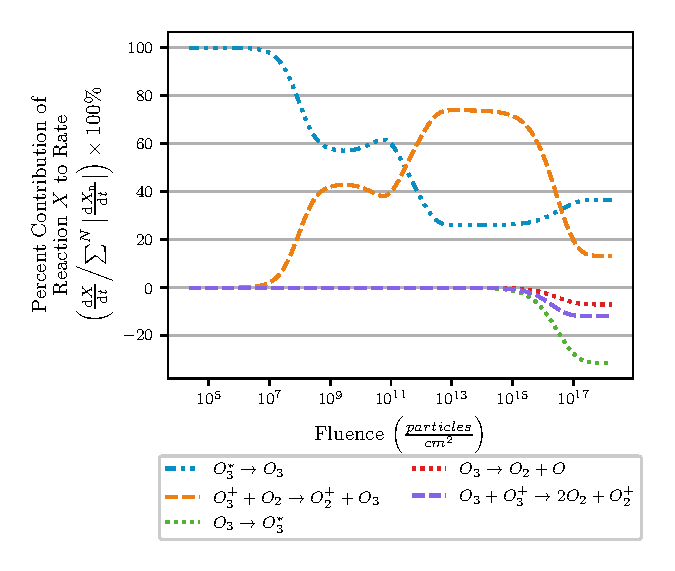
\includegraphics[width=0.5\textwidth]{Figures/bO3_rxn_contribution.eps}
%         \caption{Relative importance of formation and destruction reactions for \ce{O3}. See Table \ref{tbl:legend} for an explanation of the different linestyles.}
%         \label{fig:othreerxn}
% \end{figure}

\begin{figure}[h]
    \centering
    \begin{subfigure}[t]{0.49\textwidth}
            \centering
            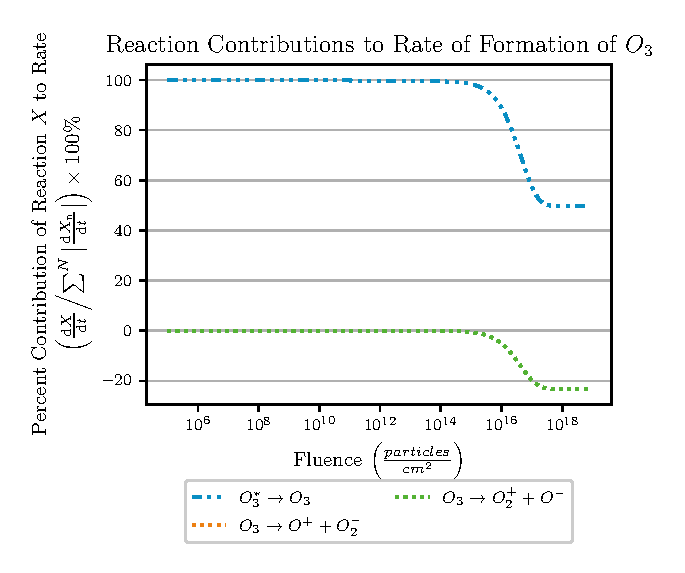
\includegraphics[width=0.9\textwidth]{Figures/bO3_rxn_contribution_noions_approx.eps}
            \caption{Model 0}
            \label{subfig:othreerxn0}
     \end{subfigure}
     \hfill
    \begin{subfigure}[t]{0.49\textwidth}
            \centering
            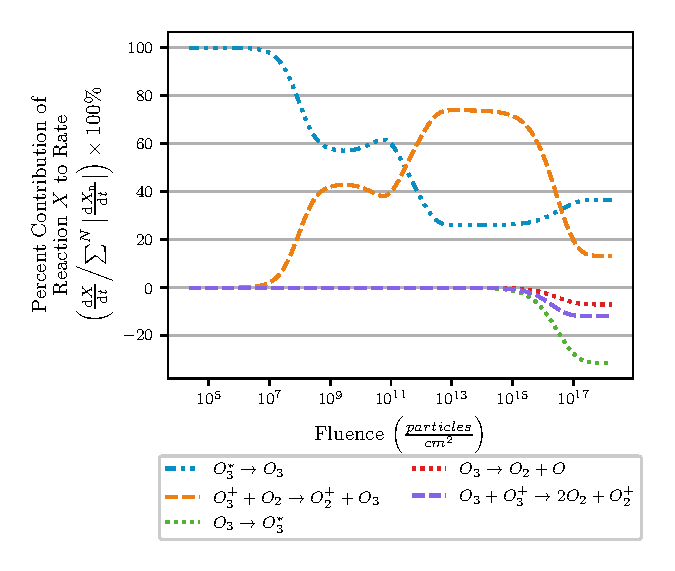
\includegraphics[width=0.9\textwidth]{Figures/bO3_rxn_contribution.eps}
            \caption{Model 1}
            \label{subfig:othreerxn1}
     \end{subfigure}
     \caption{Relative importance of formation and destruction reactions for \ce{O3}. See Table \ref{tbl:legend} for an explanation of the different linestyles. \textcolor{red}{Is this type of comparative figure useful for writing? Would having something similiar in the final paper be useful?}}
     \label{fig:othreerxn}
\end{figure}%


As shown in Fig. \ref{fig:othreerxn} \textcolor{red}{(or \ref{subfig:othreerxn1})}, at early fluences in Models 1-XXX, the rate of formation of ozone is governed by the quenching of \ce{O3^{*}}, as in Model 0.  However, at intermedia fluence values between about $10^9$ and $10^{16}$ photons/cm$^3$ the ion-neutral reaction 

\begin{equation}
    \ce{O3+ + O2 \rightarrow{} O2+ + O3}
    \tag{\ref{nlabel35}}
\end{equation}

\noindent
becomes the dominant formation pathway. At high fluences over $10^{16}$ photons/cm$^3$, the destruction of ozone is likewise primarily through the ion-neutral pathways

\begin{equation}
    \ce{O3+ + O3 \rightarrow{} 2 O2 + O2+}
    \tag{\ref{nlabel29}}
\end{equation}

\noindent
and

\begin{equation}
    \ce{O3 + O2- \rightarrow{} O2 + O3-}
    \tag{\ref{nlabel28}}
\end{equation}

\noindent
as well as via one of two photoprocesses, 

\begin{equation}
    \ce{O3  \leadsto{} O+ + O2-}
    \tag{\ref{plabel8}}
\end{equation}

\noindent
and

\begin{equation}
    \ce{O3  \leadsto{} O2+ + O-}.
    \tag{\ref{plabel10}}
\end{equation}

\noindent
The major formation and destruction reactions for the abovementioned ions are described in more detail below in \S\ref{sec:ionchemistry}. 

In Models 1-XXX, reaction \eqref{ozoneneutralformation}, the primary formation route in Model 0, contributes less than 10\% of the formation of \ce{O3} at steady state. This result again highlights the fact that, if solid phase ions do not immediately recombine, their effects on the underlying chemistry are profound.

% \begin{figure}[h]
%     \centering
%     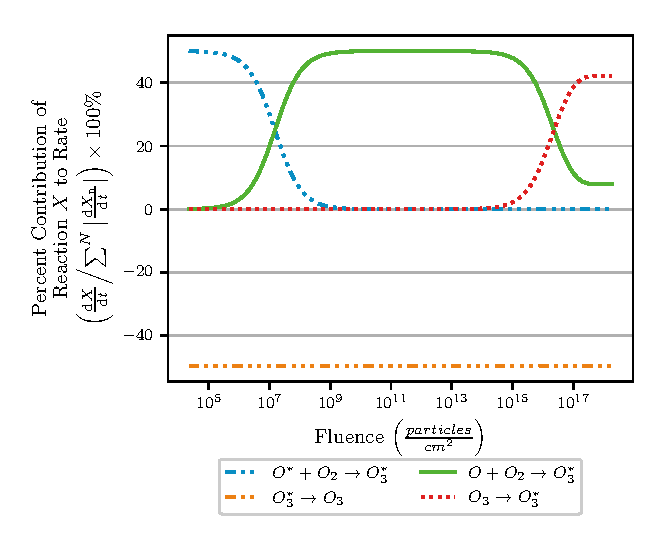
\includegraphics[width=0.5\textwidth]{Figures/bO3s_rxn_contribution.eps}
%     \caption{Relative importance of formation and destruction reactions for \ce{O3^*}. See Table \ref{tbl:legend} for an explanation of the different linestyles.}
%     \label{fig:othreesuprarxn}
% \end{figure}

\begin{figure}[h]
    \centering
    \begin{subfigure}[t]{0.49\textwidth}
            \centering
            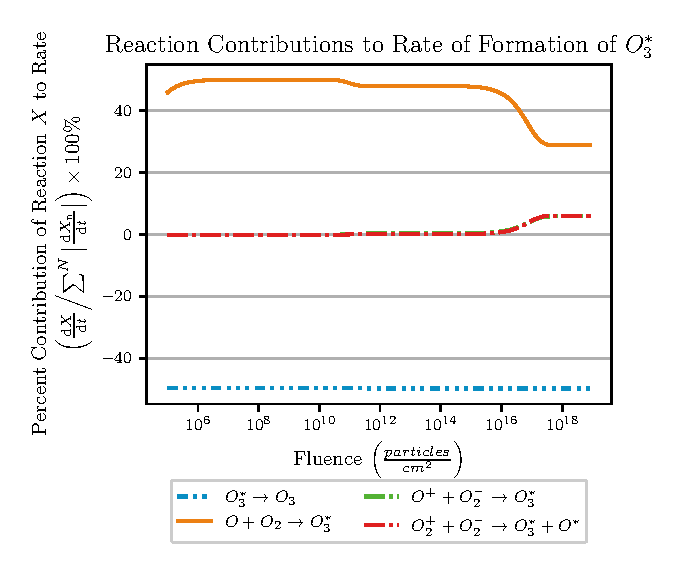
\includegraphics[width=0.9\textwidth]{Figures/bO3s_rxn_contribution_noions_approx.eps}
            \caption{Model 0}
            \label{subfig:othreesuprarxn0}
     \end{subfigure}
     \hfill
    \begin{subfigure}[t]{0.49\textwidth}
            \centering
            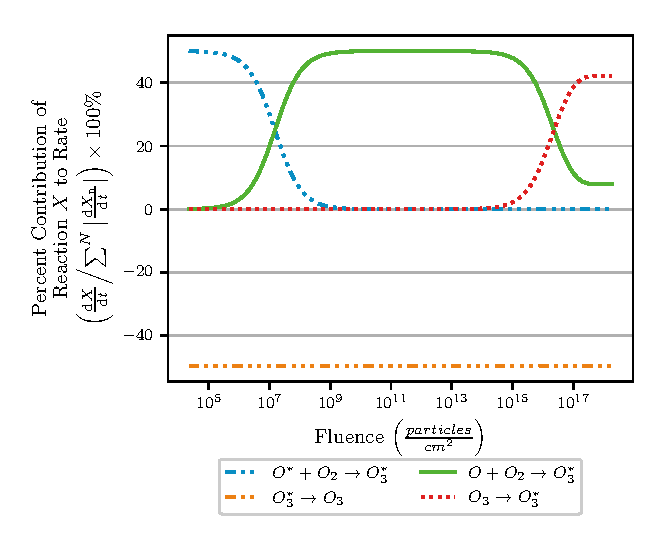
\includegraphics[width=0.9\textwidth]{Figures/bO3s_rxn_contribution.eps}
            \caption{Model 1}
            \label{subfig:othreesuprarxn1}
     \end{subfigure}
     \caption{Relative importance of formation and destruction reactions for \ce{O3^*}. See Table \ref{tbl:legend} for an explanation of the different linestyles.}
     \label{fig:othreesuprarxn}
\end{figure}%

\begin{table}
  \caption{\ce{O3} Formation at Steady State. \textbf{This table is not currently referenced in the text}\textcolor{red}{What does A+ + B- mean here? Is it a collection if reactions with similar products?} \textcolor{blue}{Yes, it's a collection of all the contributing ion-recombination reactions. Red, purple, sand, and pink in figure \ref{subfig:othreesuprarxn1}}}
  \label{tbl:othreeformation}
  \begin{tabular}{l c}
        \hline
        Reaction & \% Formation\\
        \hline
        $\ce{O3+} + \ce{O2} \rightarrow{} \ce{O2+} + \ce{O3}$ & 63.62\% \\
        $\ce{A+} + \ce{B-} \rightarrow{} \ce{O3^*} \leadsto{} \ce{O3}$ & 26.49\%  \\
        $\ce{O} + \ce{O2} \rightarrow{} \ce{O3^*} \leadsto{} \ce{O3}$ & 9.59\% \\
        \hline
    \end{tabular}
\end{table}

\subsubsection{\ce{O}}

% \begin{figure}[h]
%     \centering
%     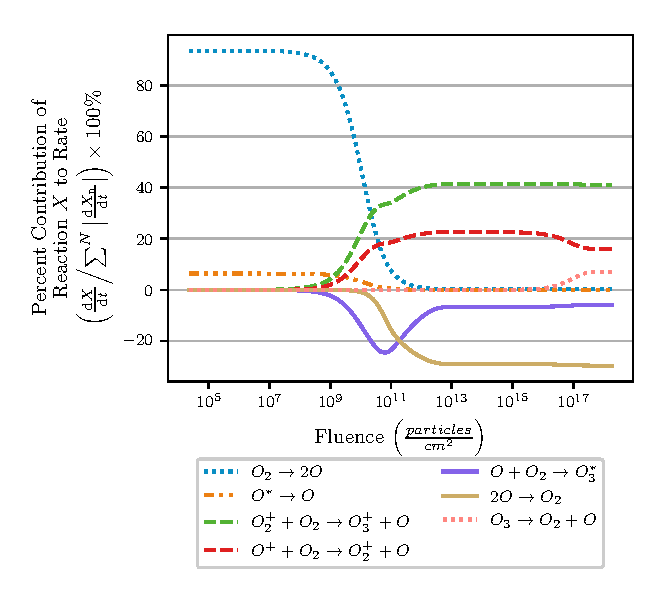
\includegraphics[width=0.5\textwidth]{Figures/bO_rxn_contribution.eps}
%     \caption{Relative importance of formation and destruction reactions for atomic oxygen. See Table \ref{tbl:legend} for an explanation of the different linestyles.}
%     \label{fig:orxn}
% \end{figure}

\begin{figure}[h]
    \centering
    \begin{subfigure}[t]{0.49\textwidth}
            \centering
            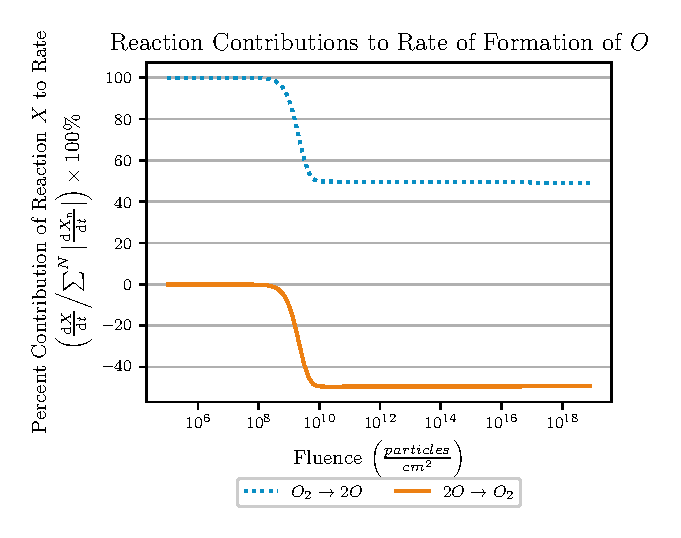
\includegraphics[width=0.9\textwidth]{Figures/bO_rxn_contribution_noions_approx.eps}
            \caption{Model 0}
            \label{subfig:orxn0}
     \end{subfigure}
     \hfill
    \begin{subfigure}[t]{0.49\textwidth}
            \centering
            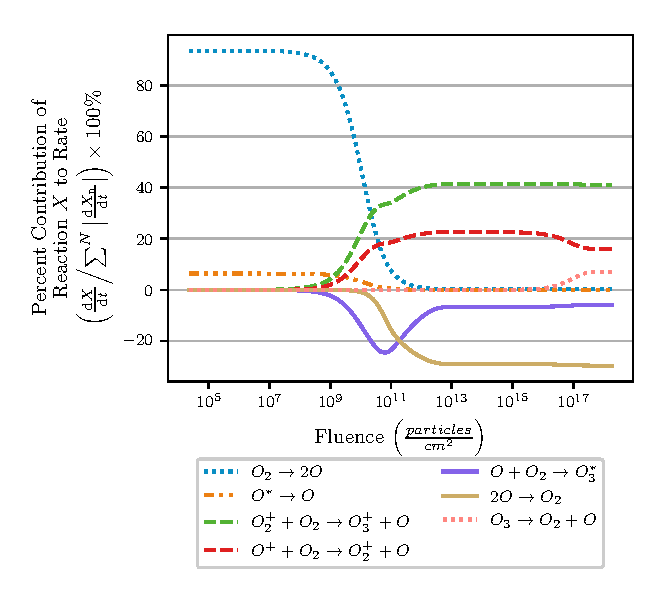
\includegraphics[width=0.9\textwidth]{Figures/bO_rxn_contribution.eps}
            \caption{Model 1}
            \label{subfig:orxn1}
     \end{subfigure}
    \caption{Relative importance of formation and destruction reactions for atomic oxygen. See Table \ref{tbl:legend} for an explanation of the different linestyles.}
    \label{fig:orxn}
\end{figure}%

In our models, the chemistry of atomic oxygen largely follows the same pattern as \ce{O3}. In Model 0, where the ion abundance is inhibited, the major formation pathway at all fluences is

\begin{equation}
    \ce{O2 \leadsto{} 2O}
    \tag{\ref{plabel3}}
    \label{oformation}
\end{equation}

\noindent
and the major destruction pathway is the reformation of molecular oxygen

\begin{equation}
    \ce{2O -> O2}
    \tag{\ref{nlabel1}}
    \label{odestruction}
\end{equation}

\noindent
However, as with \ce{O3}, in Models 1-XXX, ion-neutral reactions dominate, as can be seen in Fig. \ref{fig:orxn}. There, one can see that at early times, reaction \eqref{oformation} is most important, however, after a fluence of $10^{11}$ photons/cm$^{3}$ is reached, the reactions

\begin{equation}
    \ce{O2+ + O2 -> O3+ + O}
    \tag{\ref{nlabel20}}
    \label{otwoiondest}
\end{equation}

\noindent
and

\begin{equation}
    \ce{O+ + O2 -> O2+ + O}
    \tag{\ref{nlabel9}}
\end{equation}

\noindent
become more significant. Even in Models 1-XXX, however, reaction \eqref{odestruction} remains the major destruction pathway. 

\begin{comment}
See figure \ref{fig:orxn}. At early fluences the rate of formation of \ce{O} is governed by the photoexcitation reaction $\ce{O2 \leadsto{} 2 O}$. As more species form in the ice, the ion-neutral reactions, $\ce{O+ + O2  \rightarrow{} O2+ + O}$ and $\ce{O2+ + O2  \rightarrow{} O3+ + O}$, become the major formation pathways. The destruction pathway of \ce{O} is dominated by the neutral-neutral reaction $\ce{2O \rightarrow{} O2}$. In the neutral only model, the photoexcitation reaction $\ce{O2 \leadsto{} 2 O}$ is the only formation pathway at all fluences. 
\end{comment}

\subsubsection{\ce{O2}}


\begin{comment}
See figure \ref{fig:otworxn}.At the start of our simulations, the ice is composed of entirely \ce{O2} ice. At early fluences the primary destruction pathway is $\ce{O2 \leadsto{} 2 O}$ with some contribution from $\ce{O2  \leadsto{} O+ + O-}$. As cations form in the ice, ion-neutral reactions become the major destruction pathways so that at late fluences the major destruction pathways are $\ce{O2+ + O2 \rightarrow{} O3+ + O}$, $\ce{O+ + O2 \rightarrow{} O2+ + O}$, $\ce{O3+ + O2 \rightarrow{} 2O2 + O+}$ and $\ce{O3+ + O2 \rightarrow{} O2+ + O3}$. The primary formation pathway is the neutral-neutral reaction, $\ce{2O \rightarrow{} O2}$, with the ion-neural reaction, $\ce{O3+ + O3 \rightarrow{} 2O2 + O2+}$, and the quenching of \ce{O2^{*}} contributing non-negligibly to the formation of \ce{O2} at later fluences.
\end{comment}

% \begin{figure}[h]
%     \centering
%     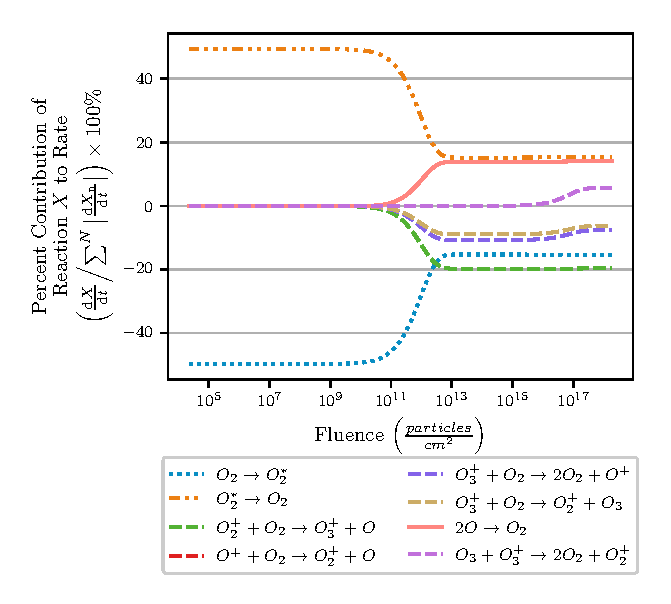
\includegraphics[width=0.5\textwidth]{Figures/bO2_rxn_contribution.eps}
%     \caption{Relative importance of formation and destruction reactions for \ce{O2}. See Table \ref{tbl:legend} for an explanation of the different linestyles.}
%     \label{fig:otworxn}
% \end{figure}

\begin{figure}[h]
    \centering
    \begin{subfigure}[t]{0.49\textwidth}
            \centering
            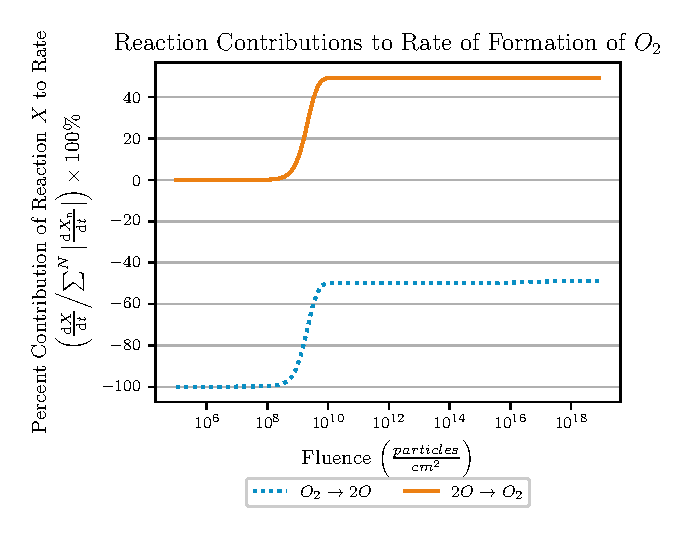
\includegraphics[width=0.9\textwidth]{Figures/bO2_rxn_contribution_noions_approx.eps}
            \caption{Model 0}
            \label{subfig:otworxn0}
     \end{subfigure}
     \hfill
    \begin{subfigure}[t]{0.49\textwidth}
            \centering
            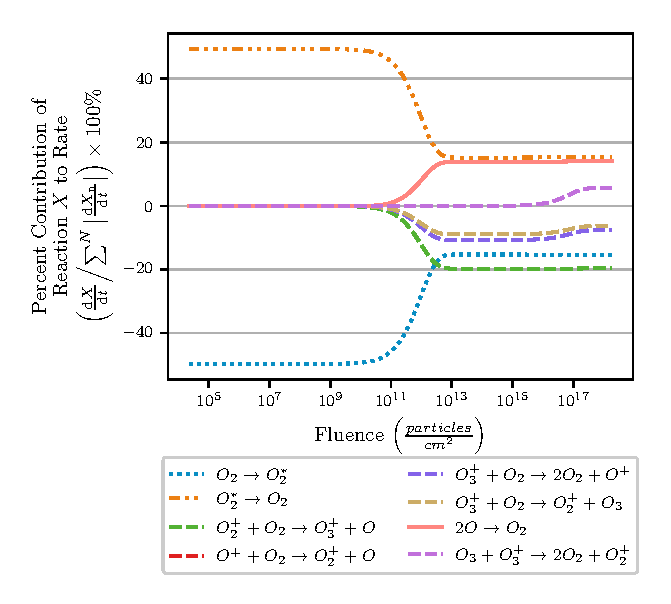
\includegraphics[width=0.9\textwidth]{Figures/bO2_rxn_contribution.eps}
            \caption{Model 1}
            \label{subfig:otworxn1}
     \end{subfigure}
    \caption{Relative importance of formation and destruction reactions for \ce{O2}. See Table \ref{tbl:legend} for an explanation of the different linestyles.}
    \label{fig:otworxn}
\end{figure}%

For \ce{O2}, the dominant formation route in all models is reaction \eqref{odestruction}. In Model 0, molecular oxygen is destroyed mainly via reaction \eqref{oformation}. As shown in Fig. \ref{fig:otworxn}, however, after fluences of $\sim10^{11}$, it is destroyed mainly via reaction \eqref{otwoiondest}. 

\FloatBarrier
\subsection{Ions}\label{sec:ionchemistry}

% \begin{figure}[h]
%     \centering
%     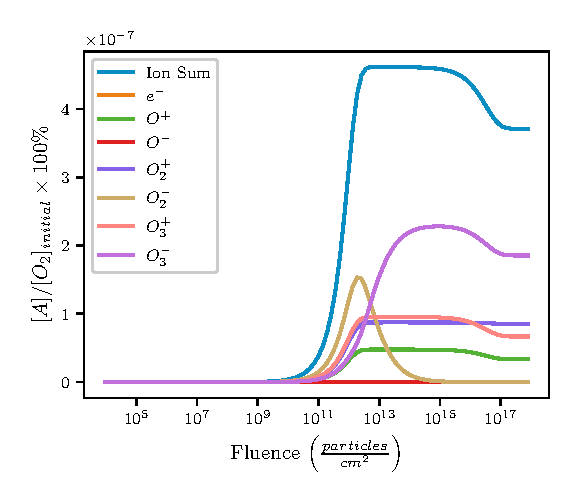
\includegraphics[width=0.5\textwidth]{Figures/ion_abundance.eps}
%     \caption{Total abundance of solid-phase ions vs. fluence.}
%     \label{fig:ionabundance}
% \end{figure}

\begin{figure}[h]
    \centering
    \begin{subfigure}[t]{0.49\textwidth}
            \centering
            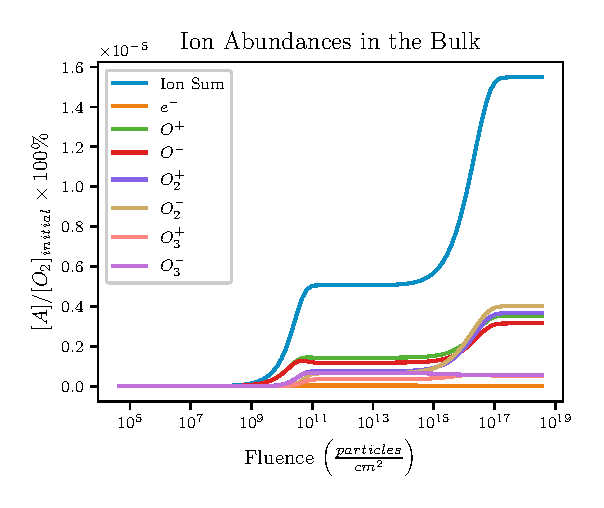
\includegraphics[width=0.9\textwidth]{Figures/ion_abundance_noions_approx.eps}
            \caption{Model 0}
            \label{subfig:ionabundance0}
     \end{subfigure}
     \hfill
    \begin{subfigure}[t]{0.49\textwidth}
            \centering
            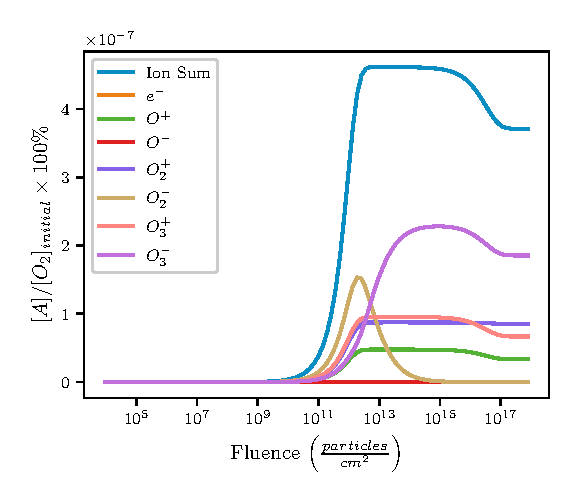
\includegraphics[width=0.9\textwidth]{Figures/ion_abundance.eps}
            \caption{Model 1}
            \label{subfig:ionabundance1}
     \end{subfigure}
     \caption{Total abundance of solid-phase ions vs. fluence.}
     \label{fig:ionabundance}
\end{figure}%

Fig. \ref{fig:ionabundance} shows the calculated abundances of the cations and anions in our simulation as a function of fluence. There one can see that the combined peak abundance of all charged species remains very low, with a value of $\sim8\times10^{-6}$\% by the end of the simulation. Here, we describe the main formation and destruction pathways of key ionic species, with more information on the rest being available in the \textit{Supplementary Information}.

% \begin{figure}[h]
%         \centering
%         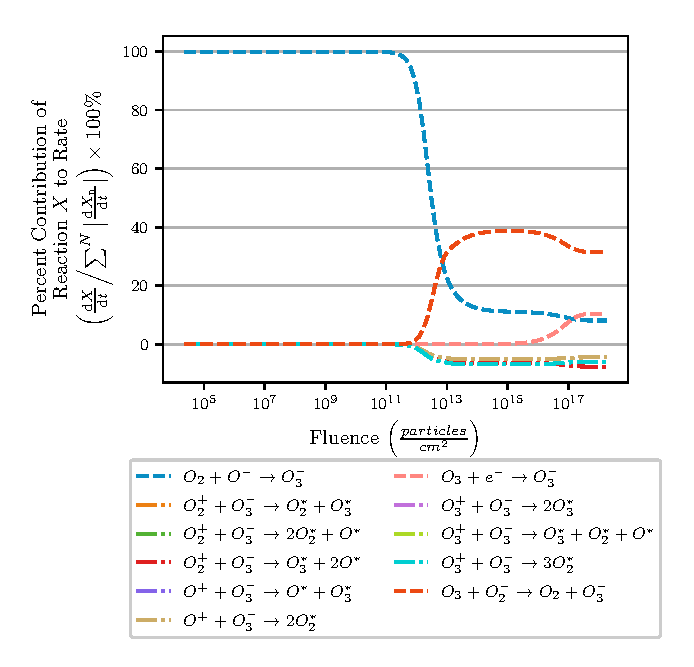
\includegraphics[width=0.5\textwidth]{Figures/bO3-_rxn_contribution.eps}
%         \caption{Relative importance of formation and destruction reactions for \ce{O3-}. See Table \ref{tbl:legend} for an explanation of the different linestyles.}
%         \label{fig:othreeminusrxn}
% \end{figure}

\begin{figure}[h]
    \centering
    \begin{subfigure}[t]{0.49\textwidth}
            \centering
            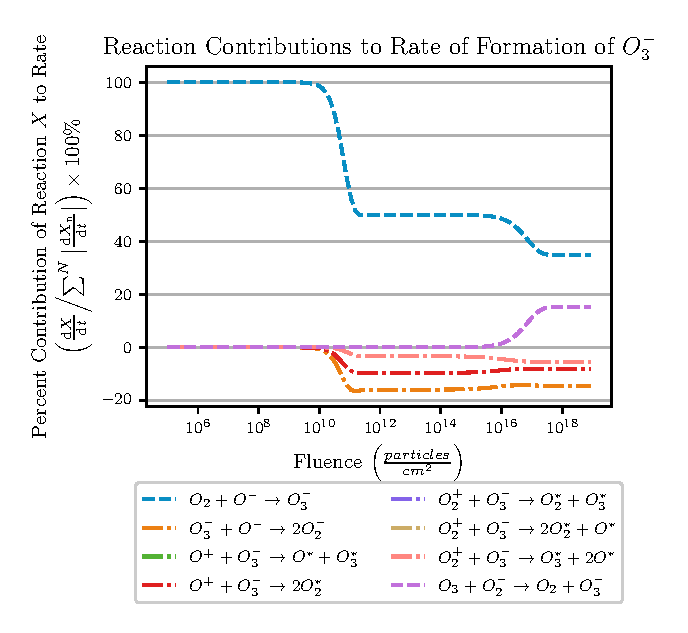
\includegraphics[width=0.9\textwidth]{Figures/bO3-_rxn_contribution_noions_approx.eps}
            \caption{Model 0}
            \label{subfig:othreeminusrxn0}
     \end{subfigure}
     \hfill
    \begin{subfigure}[t]{0.49\textwidth}
            \centering
            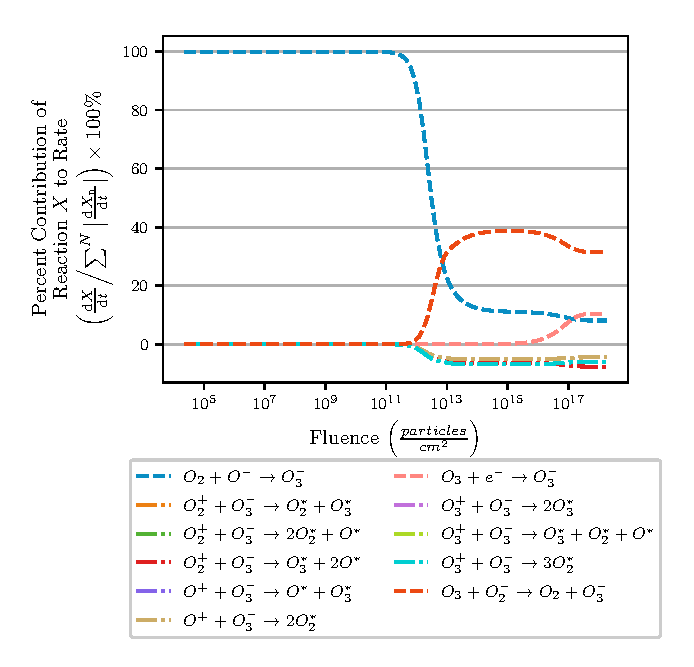
\includegraphics[width=0.9\textwidth]{Figures/bO3-_rxn_contribution.eps}
            \caption{Model 1}
            \label{subfig:othreeminusrxn1}
     \end{subfigure}
    \caption{Relative importance of formation and destruction reactions for \ce{O3-}. See Table \ref{tbl:legend} for an explanation of the different linestyles.}
    \label{fig:othreeminusrxn}
\end{figure}%

The most abundant ion at all model times is \ce{O3-}, accounting for approximately half of the total ion abundance. As shown in \ref{fig:othreeminusrxn}, at early fluences \ce{O3-} is formed via the ion-neutral reaction 

\begin{equation}
    \ce{O2 + O- \rightarrow{} O3-}
    \tag{\ref{nlabel15}}
\end{equation} 

\noindent
while at late fluences, the main formation pathway becomes

\begin{equation}
    \ce{O3 + O2- \rightarrow{} O2 + O3-}.
    \tag{\ref{nlabel28}}
\end{equation}

\noindent
The destruction of \ce{O3-} occurs entirely through ion-recombination reactions. We note that the eight ion-recombination reactions are plotted on top of each other in Fig. \ref{fig:othreeminusrxn}.


The next most abundant ionic species are \ce{O2+} and \ce{O3+}. As shown in Fig. \ref{fig:otwoplusrxn}, at early fluences the formation of \ce{O2+} proceeds mainly via the reaction

\begin{equation}
    \ce{O+ + O2 -> O2+ + O}
\end{equation}

\noindent
while the main destruction pathway is

\begin{equation}
    \ce{O2+ + O2 -> O3+ + O}.
\end{equation}

\noindent
For \ce{O3+}, the dominant formation pathway is the \ce{O2+ + O2 -> O3+ + O} reaction previously mentioned as an important formation route for atomic oxygen. 

    
    % \begin{figure}[h]
    %     \centering
    %     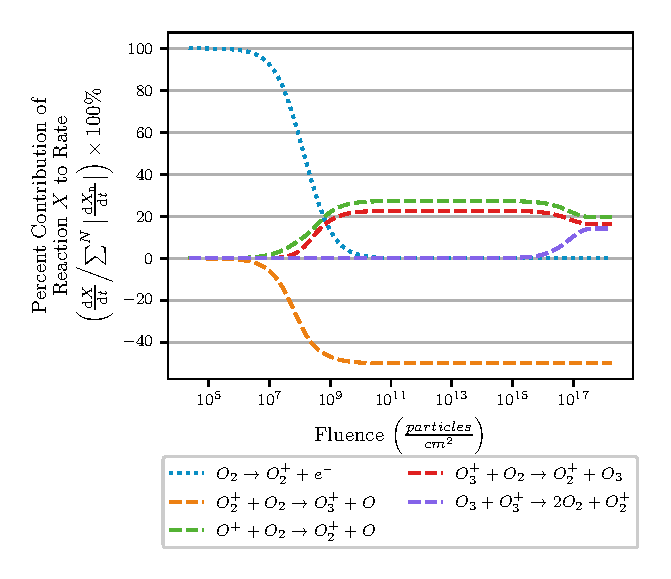
\includegraphics[width=0.5\textwidth]{Figures/bO2+_rxn_contribution.eps}
    %     \caption{Importance of \ce{O2+} reactions vs. fluence: The percent contribution of the indicated reaction to the rate of formation of \ce{O2+} with respect to $\log_{10}$ fluence. At early fluences the formation of \ce{O2+} is governed by the photoionization reaction, $\ce{O2  \leadsto{} O2+ + e-}$, quickly replace by the ion-neutral reaction, $\ce{O+ + O2  \rightarrow{} O2+ + O}$. At middle and late fluences, all major formation and destruction pathways are ion-neutral reactions.}
    %     \label{fig:otwoplusrxn}
    % \end{figure}

\begin{figure}[h]
    \centering
    \begin{subfigure}[t]{0.49\textwidth}
            \centering
            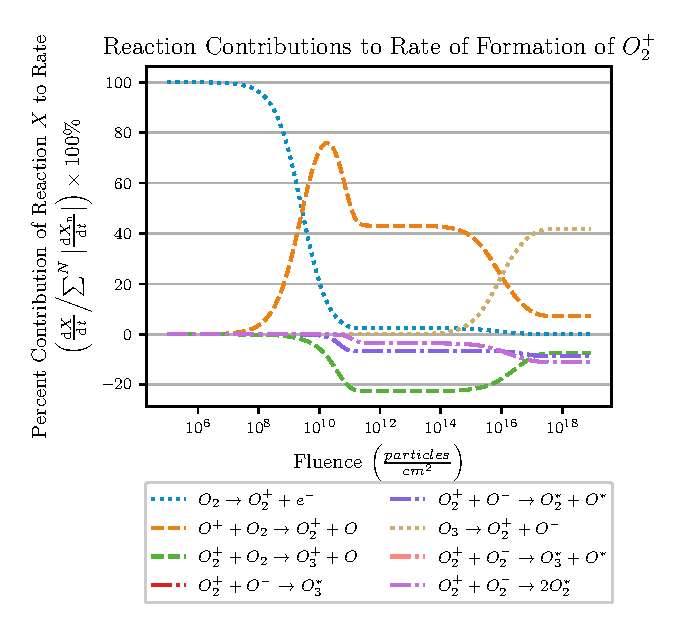
\includegraphics[width=0.9\textwidth]{Figures/bO2+_rxn_contribution_noions_approx.eps}
            \caption{Model 0}
            \label{subfig:otwoplusrxnrxn0}
     \end{subfigure}
     \hfill
    \begin{subfigure}[t]{0.49\textwidth}
            \centering
            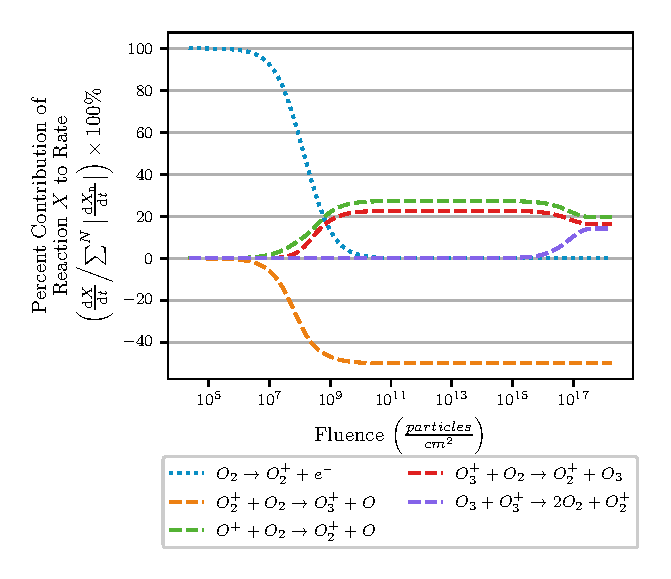
\includegraphics[width=0.9\textwidth]{Figures/bO2+_rxn_contribution.eps}
            \caption{Model 1}
            \label{subfig:otwoplusrxnrxn1}
     \end{subfigure}
    \caption{Relative importance of formation and destruction reactions for \ce{O2+} in Model 0 and Model XXX. See Table \ref{tbl:legend} for an explanation of the different linestyles.}
    \label{fig:otwoplusrxn}
\end{figure}%


    
    % \begin{figure}[h]
    %     \centering
    %     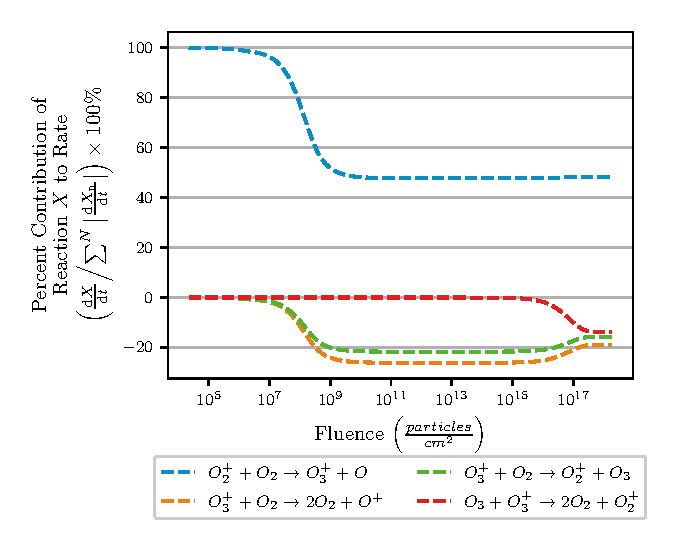
\includegraphics[width=0.5\textwidth]{Figures/bO3+_rxn_contribution.eps}
    %     \caption{Importance of \ce{O3+} reactions vs. fluence: The percent contribution of the indicated reaction to the rate of formation of \ce{O3+} with respect to $\log_{10}$ fluence. At all fluences, ion-neutral reactions are the major formation ($\ce{O2+ + O2  \rightarrow{} O3+ + O}$) and destruction ($\ce{O3+ + O2  \rightarrow{} 2O2 + O+}$, $\ce{O3+ + O2  \rightarrow{} O2+ + O3}$, and $\ce{O3+ + O3  \rightarrow{} 2O2 + O2+}$) pathways of \ce{O3+}.}
    %     \label{fig:othreeplusrxn}
    % \end{figure}

\begin{figure}[h]
    \centering
    \begin{subfigure}[t]{0.49\textwidth}
            \centering
            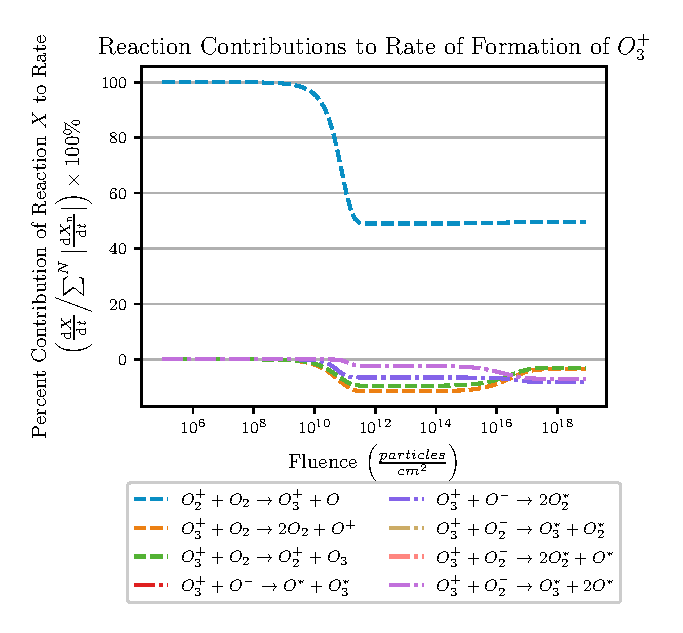
\includegraphics[width=0.9\textwidth]{Figures/bO3+_rxn_contribution_noions_approx.eps}
            \caption{Model 0}
            \label{subfig:othreeplusrxn0}
     \end{subfigure}
     \hfill
    \begin{subfigure}[t]{0.49\textwidth}
            \centering
            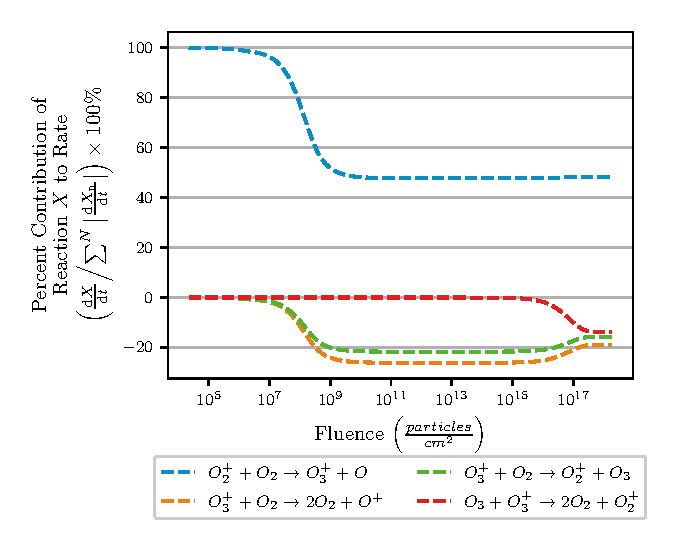
\includegraphics[width=0.9\textwidth]{Figures/bO3+_rxn_contribution.eps}
            \caption{Model 1}
            \label{subfig:othreeplusrxn1}
     \end{subfigure}
    \caption{Relative importance of formation and destruction reactions for \ce{O3+} in Model 0 and Model 1. See Table \ref{tbl:legend} for an explanation of the different linestyles.}
    \label{fig:othreeplusrxn}
\end{figure}%
           

\begin{comment}
    \paragraph{\ce{o+}}
    
    see figure \ref{fig:oplusrxn}. at early fluences the formation of \ce{o+} is governed by the photoexcitation reaction, $\ce{o2  \leadsto{} o+ + o-}$. at steady state both major formation and destruction pathways are ion-neutral reactions, $\ce{o3+ + o2  \rightarrow{} 2 o2 + o+}$ and $\ce{o+ + o2  \rightarrow{} o2+ + o}$.

    \begin{figure}[h]
        \centering
        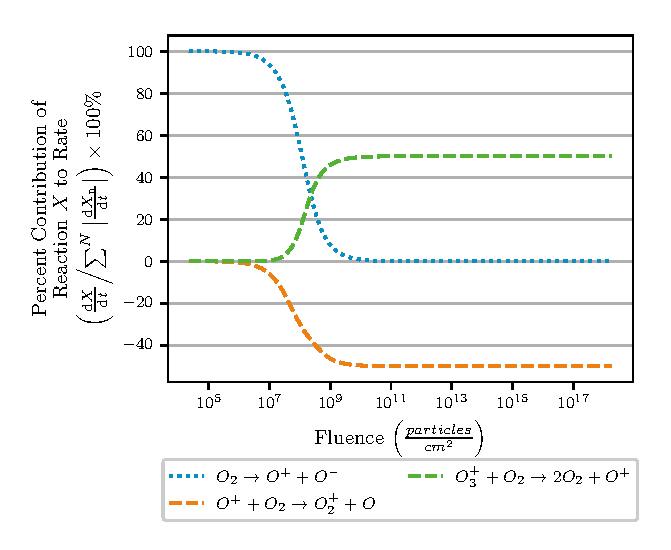
\includegraphics[width=0.5\textwidth]{Figures/bO+_rxn_contribution.eps}
        \caption{Importance of \ce{O+} reactions vs. fluence: The percent contribution of the indicated reaction to the rate of formation of \ce{O+} with respect to $\log_{10}$ fluence. At early fluences the formation of \ce{O+} is governed by the photoexcitation reaction, $\ce{O2  \leadsto{} O+ + O-}$. At steady state both major formation and destruction pathways are ion-neutral reactions, $\ce{O3+ + O2  \rightarrow{} 2 O2 + O+}$ and $\ce{O+ + O2  \rightarrow{} O2+ + O}$.}
        \label{fig:oplusrxn}
    \end{figure}
\end{comment}


	 \FloatBarrier
    \subsubsection{Electrons}



    

     See figure \ref{fig:erxn}. Electrons are entirely produced in the photoionization of \ce{O2}, $\ce{O2} \leadsto{} \ce{O2+} + \ce{e-}$. They are consumed in ion-neutral reactions with \ce{O2} and \ce{O3}.    

    % \begin{figure}[h]
    %     \centering
    %     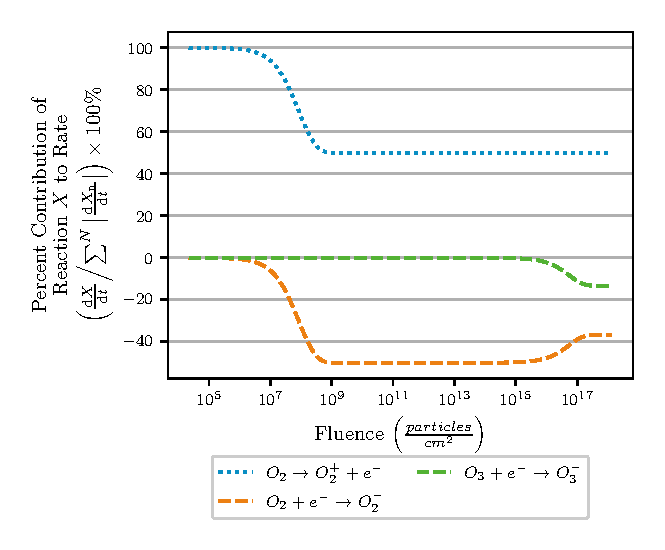
\includegraphics[width=0.5\textwidth]{Figures/be-_rxn_contribution.eps}
    %     \caption{Importance of electron reactions vs. fluence: The percent contribution of the indicated reaction to the rate of formation of \ce{e-} with respect to $\log_{10}$ fluence. Electrons are entirely produced in the photoionization of \ce{O2}, $\ce{O2} \leadsto{} \ce{O2+} + \ce{e-}$. They are consumed in ion-neutral reactions with \ce{O2} and \ce{O3}.}
    %     \label{fig:erxn}
    % \end{figure}

\begin{figure}[h]
    \centering
    \begin{subfigure}[t]{0.49\textwidth}
            \centering
            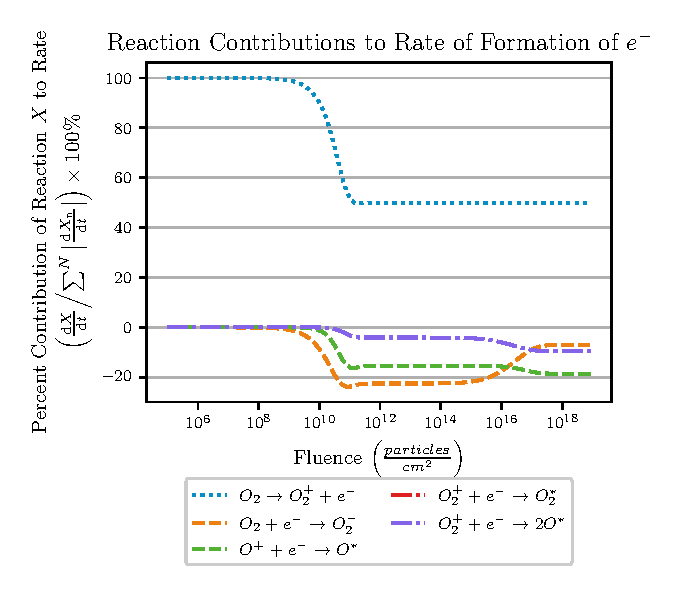
\includegraphics[width=0.9\textwidth]{Figures/be-_rxn_contribution_noions_approx.eps}
            \caption{Model 0}
            \label{subfig:erxn0}
     \end{subfigure}
     \hfill
    \begin{subfigure}[t]{0.49\textwidth}
            \centering
            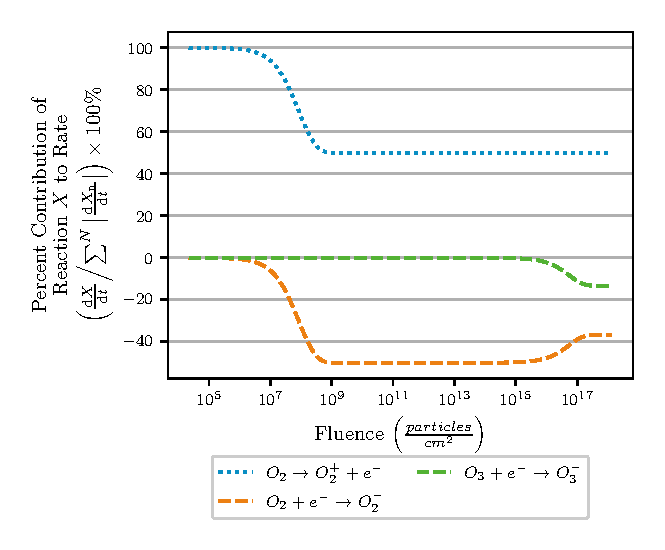
\includegraphics[width=0.9\textwidth]{Figures/be-_rxn_contribution.eps}
            \caption{Model 1}
            \label{subfig:erxn1}
     \end{subfigure}
    \caption{Importance of electron reactions vs. fluence: The percent contribution of the indicated reaction to the rate of formation of \ce{e-} with respect to $\log_{10}$ fluence. Electrons are entirely produced in the photoionization of \ce{O2}, $\ce{O2} \leadsto{} \ce{O2+} + \ce{e-}$. They are consumed in ion-neutral reactions with \ce{O2} and \ce{O3}.}
    \label{fig:erxn}
\end{figure}%
           

    \paragraph{\ce{O-}}

     See figure \ref{fig:ominusrxn}. The formation of \ce{O-} is governed by photoexcitation reactions. At early fluences it is the photodissociation of \ce{O2}, $\ce{O2  \leadsto{} O+ + O-}$, but at steady state it is the photodissociation of \ce{O3}, $\ce{O3  \leadsto{} O2+ + O-}$. Both major destruction pathways are ion-neutral reactions, $\ce{O2 + O- \rightarrow{} O3-}$ and $\ce{O3 + O- \rightarrow{} O2 + O2-}$.

    % \begin{figure}[h]
    %     \centering
    %     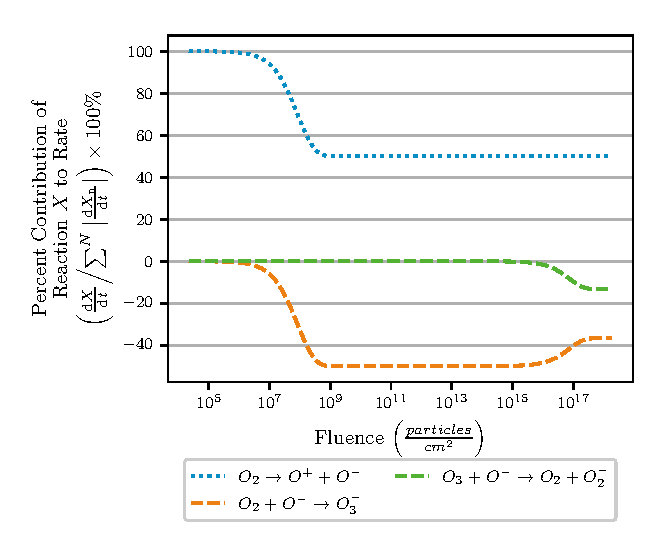
\includegraphics[width=0.5\textwidth]{Figures/bO-_rxn_contribution.eps}
    %     \caption{Importance of \ce{O-} reactions vs. fluence: The percent contribution of the indicated reaction to the rate of formation of \ce{O-} with respect to $\log_{10}$ fluence. The formation of \ce{O-} is governed by photoexcitation reactions. At early fluences it is the photodissociation of \ce{O2}, $\ce{O2  \leadsto{} O+ + O-}$, but at steady state it is the photodissociation of \ce{O3}, $\ce{O3  \leadsto{} O2+ + O-}$. Both major destruction pathways are ion-neutral reactions, $\ce{O2 + O- \rightarrow{} O3-}$ and $\ce{O3 + O- \rightarrow{} O2 + O2-}$.}
    %     \label{fig:ominusrxn}
    % \end{figure}

    \begin{figure}[h]
    \centering
    \begin{subfigure}[t]{0.49\textwidth}
            \centering
            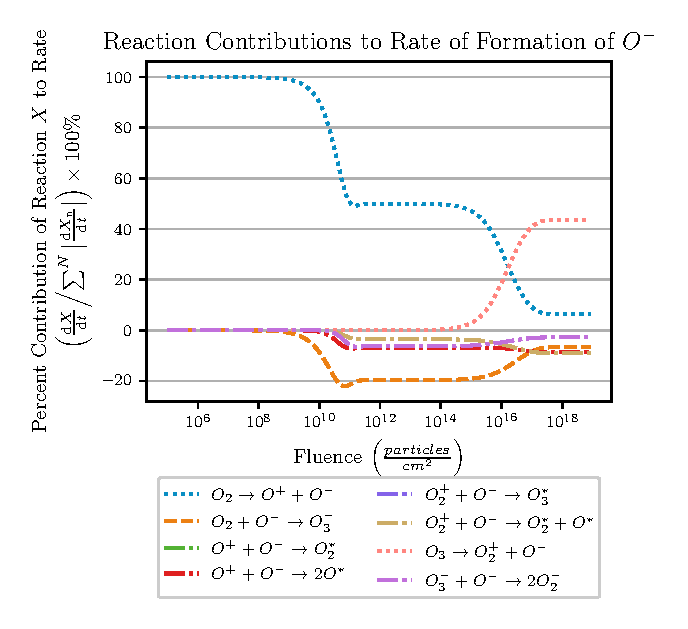
\includegraphics[width=0.9\textwidth]{Figures/bO-_rxn_contribution_noions_approx.eps}
            \caption{Model 0}
            \label{subfig:ominusrxn0}
     \end{subfigure}
     \hfill
    \begin{subfigure}[t]{0.49\textwidth}
            \centering
            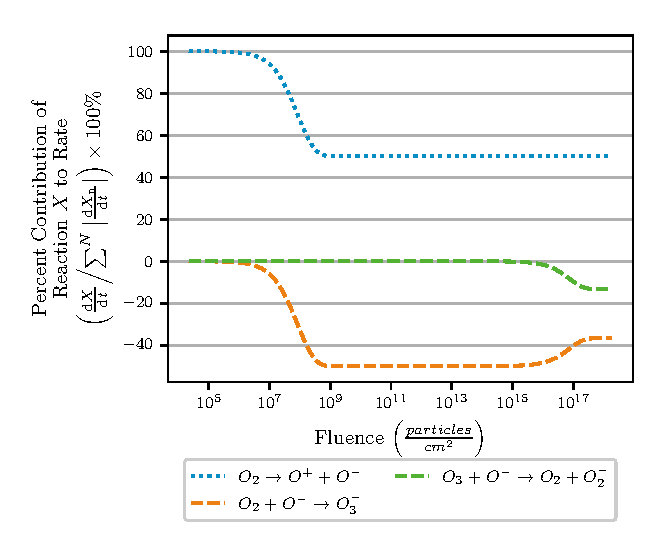
\includegraphics[width=0.9\textwidth]{Figures/bO-_rxn_contribution.eps}
            \caption{Model 1}
            \label{subfig:ominusrxn1}
     \end{subfigure}
        \caption{Importance of \ce{O-} reactions vs. fluence: The percent contribution of the indicated reaction to the rate of formation of \ce{O-} with respect to $\log_{10}$ fluence. The formation of \ce{O-} is governed by photoexcitation reactions. At early fluences it is the photodissociation of \ce{O2}, $\ce{O2  \leadsto{} O+ + O-}$, but at steady state it is the photodissociation of \ce{O3}, $\ce{O3  \leadsto{} O2+ + O-}$. Both major destruction pathways are ion-neutral reactions, $\ce{O2 + O- \rightarrow{} O3-}$ and $\ce{O3 + O- \rightarrow{} O2 + O2-}$.}
        \label{fig:ominusrxn}
    \end{figure}%

    \paragraph{\ce{O2-}}

     See figure \ref{fig:otwominusrxn}. At early fluences \ce{O2-} is formed via the ion-neutral reaction, $\ce{O2 + e- \rightarrow{} O2-}$, but as more species are formed the photodissociation of \ce{O3}, $\ce{O3  \leadsto{} O+ + O2-}$, becomes the major formation pathway. Destruction pathways are primarially ion-recombination reactions until late fluences when the ion-neutral reaction, $\ce{O3 + O2- \rightarrow{} O2 + O3-}$, dominates.
    
    % \begin{figure}[h]
    %     \centering
    %     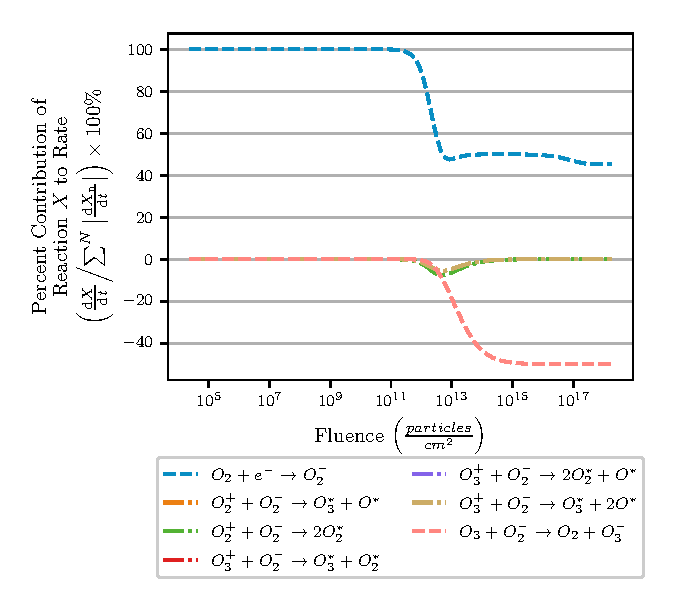
\includegraphics[width=0.5\textwidth]{Figures/bO2-_rxn_contribution.eps}
    %     \caption{Importance of \ce{O2-} reactions vs. fluence: The percent contribution of the indicated reaction to the rate of formation of \ce{O2-} with respect to $\log_{10}$ fluence. At early fluences \ce{O2-} is formed via the ion-neutral reaction, $\ce{O2 + e- \rightarrow{} O2-}$, but as more species are formed the photodissociation of \ce{O3}, $\ce{O3  \leadsto{} O+ + O2-}$, becomes the major formation pathway. Destruction pathways are primarially ion-recombination reactions until late fluences when the ion-neutral reaction, $\ce{O3 + O2- \rightarrow{} O2 + O3-}$, dominates.}
    %     \label{fig:otwominusrxn}
    % \end{figure}

\begin{figure}[h]
    \centering
    \begin{subfigure}[t]{0.49\textwidth}
            \centering
            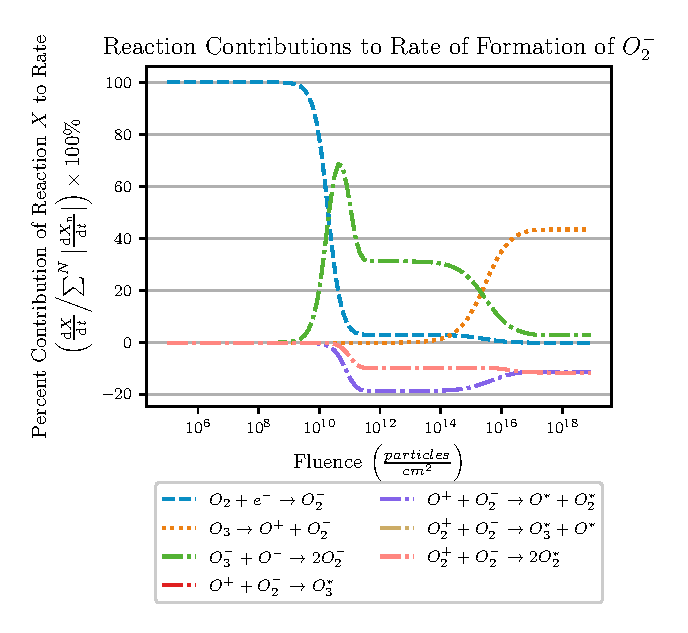
\includegraphics[width=0.9\textwidth]{Figures/bO2-_rxn_contribution_noions_approx.eps}
            \caption{Model 0}
            \label{subfig:otwominusrxn0}
     \end{subfigure}
     \hfill
    \begin{subfigure}[t]{0.49\textwidth}
            \centering
            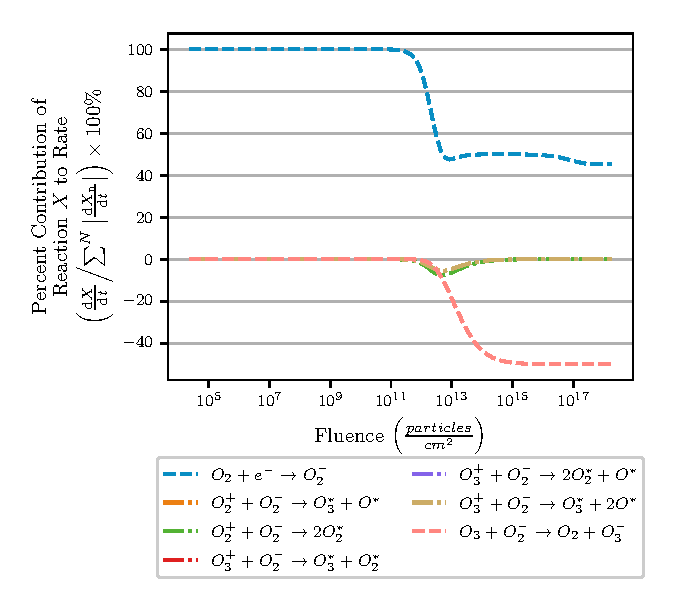
\includegraphics[width=0.9\textwidth]{Figures/bO2-_rxn_contribution.eps}
            \caption{Model 1}
            \label{subfig:otwominusrxn1}
     \end{subfigure}
    \caption{Importance of \ce{O2-} reactions vs. fluence: The percent contribution of the indicated reaction to the rate of formation of \ce{O2-} with respect to $\log_{10}$ fluence. At early fluences \ce{O2-} is formed via the ion-neutral reaction, $\ce{O2 + e- \rightarrow{} O2-}$, but as more species are formed the photodissociation of \ce{O3}, $\ce{O3  \leadsto{} O+ + O2-}$, becomes the major formation pathway. Destruction pathways are primarially ion-recombination reactions until late fluences when the ion-neutral reaction, $\ce{O3 + O2- \rightarrow{} O2 + O3-}$, dominates.}
    \label{fig:otwominusrxn}
\end{figure}%


\FloatBarrier
    \subsubsection{Sensitivity Analysis}
    
    The RMSD fit of the model is not sensitive to changes in  $\nu_{n-n}$. The RMSD fit of the model is highly sensitive to changes in the ratio of $\nu_{i-i}/\nu_{i-n}$. See Figure \ref{fig:sensitivityionionnuionnu}. 

    The ion-abundance at steady state did not clearly correlate with the $\nu_{i-i}/\nu_{i-n}$ ratio, nor with $\nu_{i-i}$ or $\nu_{i-n}$ independently. 
    

    \begin{figure}
        \centering
        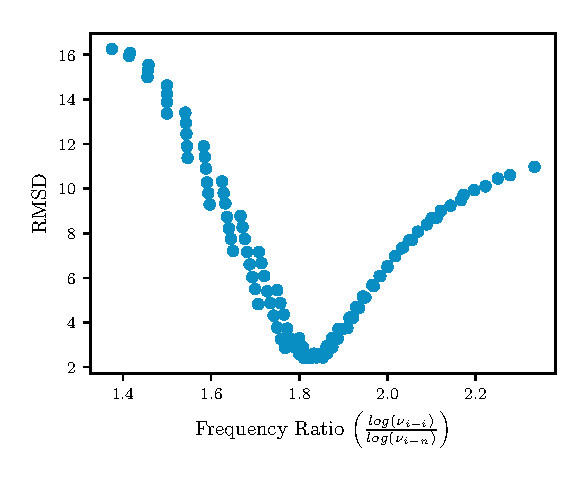
\includegraphics[width=0.5\textwidth]{Figures/ion_ratio_sensitivity.eps}
        \caption{Sensitivity of the model to changes in the ratio of $\log(\nu_{i-i})/\log(\nu_{i-n})$}
        \label{fig:sensitivityionionnuionnu}
    \end{figure}

    \begin{figure}
        \centering
        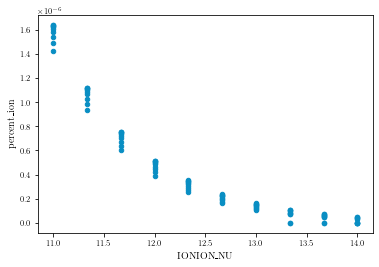
\includegraphics[width=0.5\textwidth]{Figures/ionionnu_vs_ionabundance.png}
        \caption{Sensitivity of the modeled ion abundance to changes in $\log(\nu_{i-i})$}
        \label{fig:sensitivity}
    \end{figure}

    \begin{figure}
        \centering
        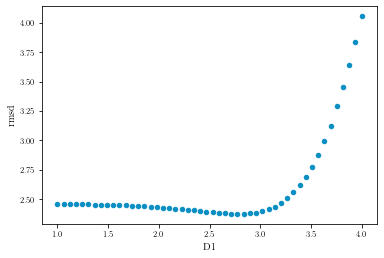
\includegraphics[width=0.5\textwidth]{Figures/D1_vs_rmsd.png}
        \caption{Sensitivity of the model to changes in the delta value for $\ce{O2 \leadsto{} 2 O}$}
        \label{fig:sensitivity}
    \end{figure}

    \begin{figure}
        \centering
        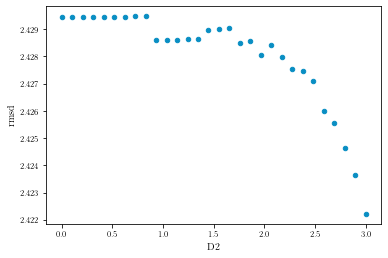
\includegraphics[width=0.5\textwidth]{Figures/D2_vs_rmsd.png}
        \caption{Sensitivity of the model to changes in the delta value for $\ce{O2 \leadsto{} 2 O^{*}}$}
        \label{fig:sensitivity}
    \end{figure}

    \begin{figure}
        \centering
        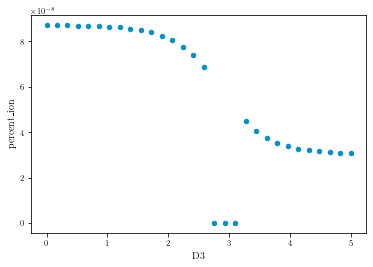
\includegraphics[width=0.5\textwidth]{Figures/D3_vs_ionabundance.png}
        \caption{Sensitivity of the modeled ion abundance to changes in the delta value for $\ce{O2 \leadsto{} 2 O*}$, $ \ce{O3 \leadsto{} O2 + O}$, and $\ce{O3 \leadsto{} O3*}$}
        \label{fig:sensitivity}
    \end{figure}

    \begin{figure}
        \centering
        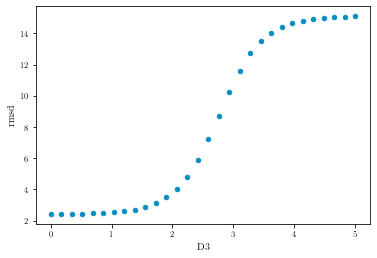
\includegraphics[width=0.5\textwidth]{Figures/D3_vs_rmsd.png}
        \caption{Sensitivity of the model to changes in the delta value for $\ce{O2 \leadsto{} 2 O*}$, $ \ce{O3 \leadsto{} O2 + O}$, and $\ce{O3 \leadsto{} O3*}$}
        \label{fig:sensitivity}
    \end{figure}

\FloatBarrier
\subsection{Conclusions} \label{sec:conclusions}






%%%%%%%%%%%%%%%%%%%%%%%%%%%%%%%%%%%%%%%%%%%%%%%%%%%%%%%%%%%%%%%%%%%%%
%% The "Acknowledgement" section can be given in all manuscript
%% classes.  This should be given within the "acknowledgement"
%% environment, which will make the correct section or running title.
%%%%%%%%%%%%%%%%%%%%%%%%%%%%%%%%%%%%%%%%%%%%%%%%%%%%%%%%%%%%%%%%%%%%%
\begin{acknowledgement}



\end{acknowledgement}

%%%%%%%%%%%%%%%%%%%%%%%%%%%%%%%%%%%%%%%%%%%%%%%%%%%%%%%%%%%%%%%%%%%%%
%% The same is true for Supporting Information, which should use the
%% suppinfo environment.
%%%%%%%%%%%%%%%%%%%%%%%%%%%%%%%%%%%%%%%%%%%%%%%%%%%%%%%%%%%%%%%%%%%%%
\FloatBarrier
\begin{suppinfo}

    % \begin{figure}[h]
    %     \centering
    %     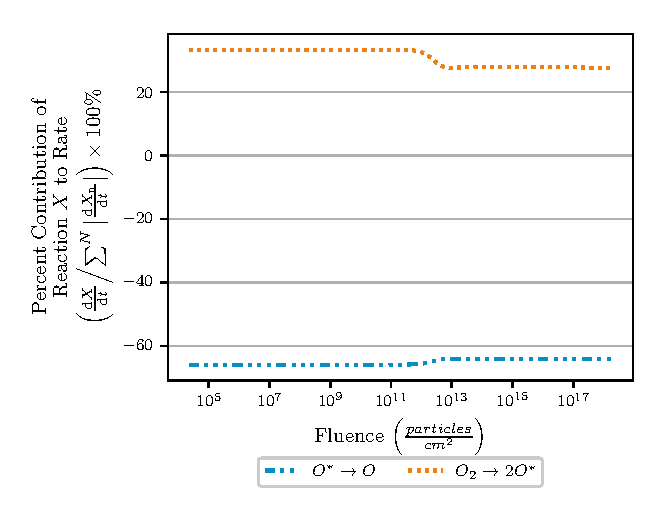
\includegraphics[width=0.5\textwidth]{Figures/bOs_rxn_contribution.eps}
    %     \caption{Importance of \ce{O^*} reactions vs. fluence:}
    %     \label{fig:osuprarxn}
    % \end{figure}

\begin{figure}[h]
    \centering
    \begin{subfigure}[t]{0.49\textwidth}
            \centering
            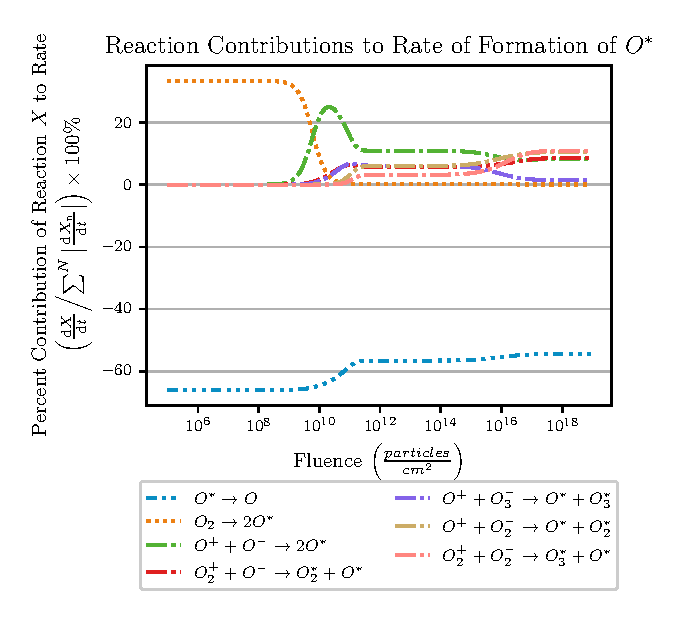
\includegraphics[width=0.9\textwidth]{Figures/bOs_rxn_contribution_noions_approx.eps}
            \caption{Model 0}
            \label{subfig:osuprarxn0}
     \end{subfigure}
     \hfill
    \begin{subfigure}[t]{0.49\textwidth}
            \centering
            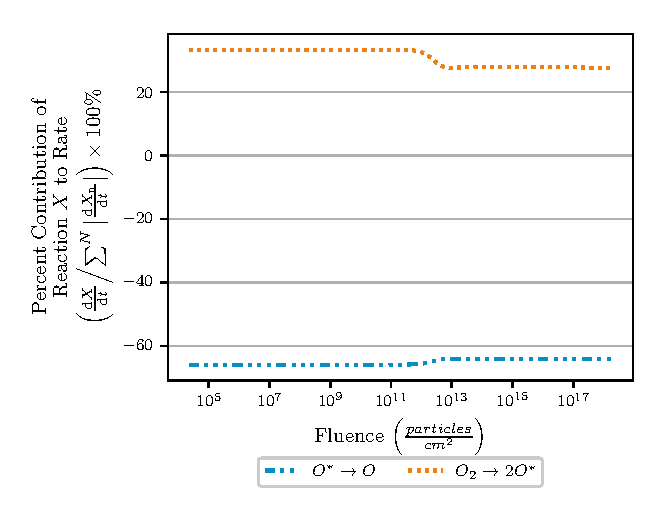
\includegraphics[width=0.9\textwidth]{Figures/bOs_rxn_contribution.eps}
            \caption{Model 1}
            \label{subfig:osuprarxn1}
     \end{subfigure}
    \caption{Importance of \ce{O^*} reactions vs. fluence:}
    \label{fig:osuprarxn}
\end{figure}%

    % \begin{figure}[h]
    %     \centering
    %     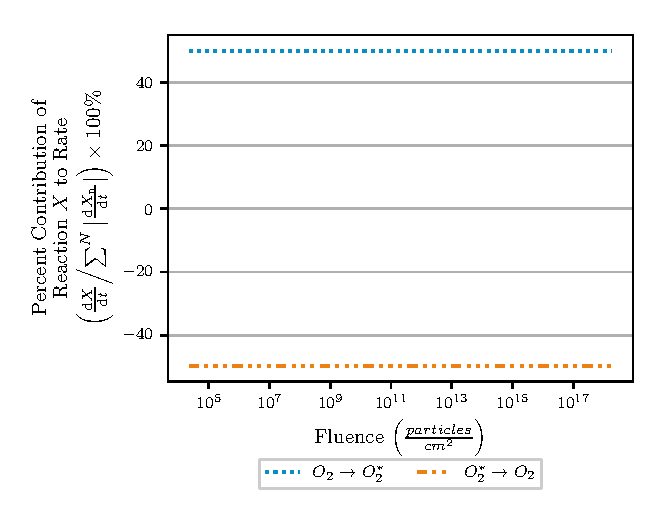
\includegraphics[width=0.5\textwidth]{Figures/bO2s_rxn_contribution.eps}
    %     \caption{Importance of \ce{O2^*} reactions vs. fluence:}
    %     \label{fig:otwosuprarxn}
    % \end{figure}

\begin{figure}[h]
    \centering
    \begin{subfigure}[t]{0.49\textwidth}
            \centering
            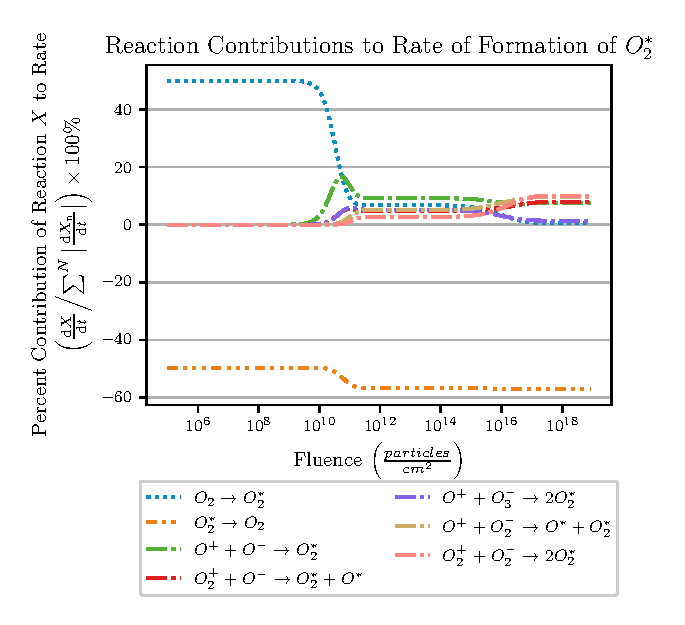
\includegraphics[width=0.9\textwidth]{Figures/bO2s_rxn_contribution_noions_approx.eps}
            \caption{Model 0}
            \label{subfig:otwosuprarxn0}
     \end{subfigure}
     \hfill
    \begin{subfigure}[t]{0.49\textwidth}
            \centering
            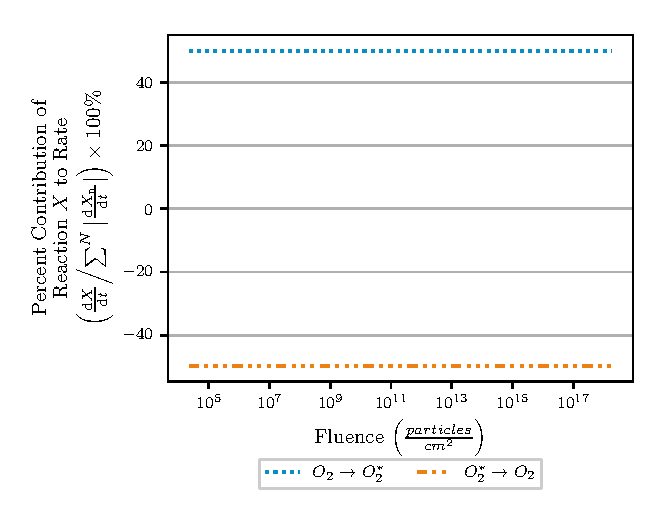
\includegraphics[width=0.9\textwidth]{Figures/bO2s_rxn_contribution.eps}
            \caption{Model 1}
            \label{subfig:otwosuprarxn1}
     \end{subfigure}
        \caption{Importance of \ce{O2^*} reactions vs. fluence:}
        \label{fig:otwosuprarxn}
\end{figure}%

\end{suppinfo}
\FloatBarrier

%%%%%%%%%%%%%%%%%%%%%%%%%%%%%%%%%%%%%%%%%%%%%%%%%%%%%%%%%%%%%%%%%%%%%
%% The appropriate \bibliography command should be placed here.
%% Notice that the class file automatically sets \bibliographystyle
%% and also names the section correctly.
%%%%%%%%%%%%%%%%%%%%%%%%%%%%%%%%%%%%%%%%%%%%%%%%%%%%%%%%%%%%%%%%%%%%%
\bibliography{references}

\end{document}